\documentclass[a4paper]{article}

%% Language and font encodings
\usepackage[english]{babel}
\usepackage[utf8x]{inputenc}
\usepackage[T1]{fontenc}

%% Sets page size and margins
\usepackage[a4paper,top=3cm,bottom=2cm,left=3cm,right=3cm,marginparwidth=1.75cm]{geometry}

%% Useful packages
\usepackage{amsmath}
\usepackage[table,xcdraw]{xcolor}
\usepackage{graphicx}
\usepackage[colorinlistoftodos]{todonotes}
\usepackage[colorlinks=true, allcolors=blue]{hyperref}
\usepackage{amsmath}
\usepackage{tikz}
\usepackage{tkz-tab}
\usepackage{caption}
\usepackage{latexsym}
\usepackage{amssymb}
\usepackage{amsmath}
\usepackage{subcaption}
\usepackage{mathtools}
\usepackage{multirow}
\usepackage{listings}
\usepackage{color}
\usepackage{epsfig}
\usepackage{epstopdf}

\definecolor{mygreen}{rgb}{0,0.6,0}
\definecolor{mygray}{rgb}{0.5,0.5,0.5}
\definecolor{mymauve}{rgb}{0.58,0,0.82}

\lstdefinestyle{customc}{
  belowcaptionskip=1\baselineskip,
  breaklines=true,
  frame=L,
  xleftmargin=\parindent,
  language=C,
  showstringspaces=false,
  basicstyle=\footnotesize\ttfamily,
  keywordstyle=\bfseries\color{green!40!black},
  commentstyle=\itshape\color{purple!40!black},
  identifierstyle=\color{blue},
  stringstyle=\color{orange},
}

\lstdefinestyle{customasm}{
  belowcaptionskip=1\baselineskip,
  frame=L,
  xleftmargin=\parindent,
  language=[x86masm]Assembler,
  basicstyle=\footnotesize\ttfamily,
  commentstyle=\itshape\color{purple!40!black},
}

\lstset{escapechar=@,style=customc}

\usetikzlibrary{automata,arrows,positioning,calc}
\usetikzlibrary{shapes,snakes}
\DeclarePairedDelimiter\abs{\lvert}{\rvert}

\title{[TUTORIAL] KOMONDOR: A Wireless Network Simulator Based for Next-Generation IEEE 802.11ax WLANs}
\author{Sergio Barrachina and Francesc Wilhelmi}

\begin{document}
\maketitle

\begin{abstract}
Komondor is a wireless network simulator that includes novel mechanisms for next-generation WLANs, such as Dynamic Channel Bonding or enhanced Spatial Reuse. One of Komondor's main purposes is to emulate the behavior of IEEE 802.11ax-2019 networks, which main challenge is spectral efficiency in dense deployments. Furthermore, due to the growing popularity of autonomous systems and the tendency of WLANs to use learning, Komondor is intended to include intelligent agents that perform operations like Carrier Sense Threshold adjustment.
\end{abstract}

\tableofcontents

\listoffigures

\listoftables

%%%%%%%%%%%%%%%
% 1. INTRODUCTION
%%%%%%%%%%%%%%%
\section{Introduction}
\label{section:introduction}
	Komondor is an event-based simulator based in COST \cite{cost}, a CompC++ library to perform discrete event simulation.\footnote{COST main website: \url{http://www.ita.cs.rpi.edu/cost.html}} The presented simulator is mostly intended to reproduce the novel techniques included in the IEEE 802.11ax-2019 amendment \cite{tgax2017draft}, which is called to become a benchmark in next-generation wireless networks. For that, and due to the lack of 11ax-oriented simulators, we aim to develop Komondor. Furthermore, a key feature of our simulator is the inclusion of agents that can decide the behavior of WLANs through Reinforcement Learning (RL). Other popular simulation tools such as ns-3 lack of flexibility and adaptability towards including online learning procedures within their operation.
	
	Komondor has been developed to be an open source tool that contributes to the ongoing research in wireless networks. Henceforth, in this document we describe its main features and system model considerations, as well as some basic guidelines to run it. To provide detailed technical information regarding the development of the code is out of the scope of this document.
	
	%%%  NG WLANs
	\subsection{Next-Generation WLANs}
	\label{section:ng_wlans}
	The increasing network requirements in terms of data rate and users capacity has brought the wireless communications community to introduce novel approaches. Regarding IEEE 802.11 WLANs, the 11ax amendment is being developed to improve spectrum efficiency in high density scenarios. To accomplish that, it introduces the concept of High-Efficiency (HE) WLANs, which incorporates new mechanisms such as OFDMA, Dynamic Channel Bonding, Beamforming and Multi-User Multiple-Input Multiple-Output (MU-MIMO). Such advanced mechanisms drastically change the current operation of WLANs and have not been previously implemented with detail in other network simulators. Further information regarding the novel capabilities included in the IEEE 802.11ax standard can be found in \cite{bellalta2016ieee}.
	
	In addition to including such novel techniques, wireless networks are evolving towards autonomous management, which in many cases is achieved through Artificial Intelligence (AI). Its utilization is expected to be key in next-generation complex systems, since it allows solving (or at least approximating) computational-intensive problems. In particular, online learning has been previously applied in well-known problems such as Transmit Power Control (TPC), Carrier Sense Threshold (CST) adjustment and channel allocation \cite{wilhelmi2017implications, wilhelmi2017collaborative, maghsudi2015joint, maghsudi2015channel}. Since most of the literature that applies learning into wireless networks is theoretical in nature, there is a strong need for tools that allow implementing learning algorithms in a realistic simulation environment.	
	
	%%%  Komondor main features
	\subsection{Komondor Main Features}
	\label{section:features}
	Komondor aims to thoroughly simulate the operation of wireless networks. Henceforth, it reproduces actual transmissions on a per-packet basis. For that, nodes properties (e.g., location, transmit power, CCA threshold) are taken into account during data exchange procedures.
	
	In overview mode, Komondor is intended to simulate the following wireless networks mechanisms:
	\begin{itemize}
		\item Distributed Coordination Function (DCF)
		\item Channel Bonding (CB)
		\item Dynamic transmit power and CST adjustment
		\item MU-MIMO transmissions
		\item Directional transmissions
		\item Packet aggregation
		\item Dynamic MCS
		\item RTS/CTS and NAV allocation
	\end{itemize}

	Note, as well, that the first version of Komondor introduced by this document includes the basic operation carried out by WLANs and only implements DCF, CB, dynamic MCS and RTS/CTS.
	
	%%%  COST 
	\subsection{COST}
	\label{section:cost}
	In order to provide a deep understanding of Komondor, it is important to briefly understand the COST library, which allows building discrete interactions between components, which may represent entities like wireless nodes. Such interaction is achieved through synchronous and asynchronous events. While the former are message explicitly exchanged between components through input/output ports, the later are based on timers. In practice, components perform a set of operations until a significant event occurs. For instance, a node that is decreasing its backoff (i.e., current operation) may freeze it when an overlapping node occupies the channel (i.e., an event). Figure \ref{fig:cost} shows the schematic of a COST component, which is characterized by its inports and outports, and a set of timers. While inports and outports allow to directly communicate with other components, timers trigger events specific to the component.
	\begin{figure}[h!]
		\centering
		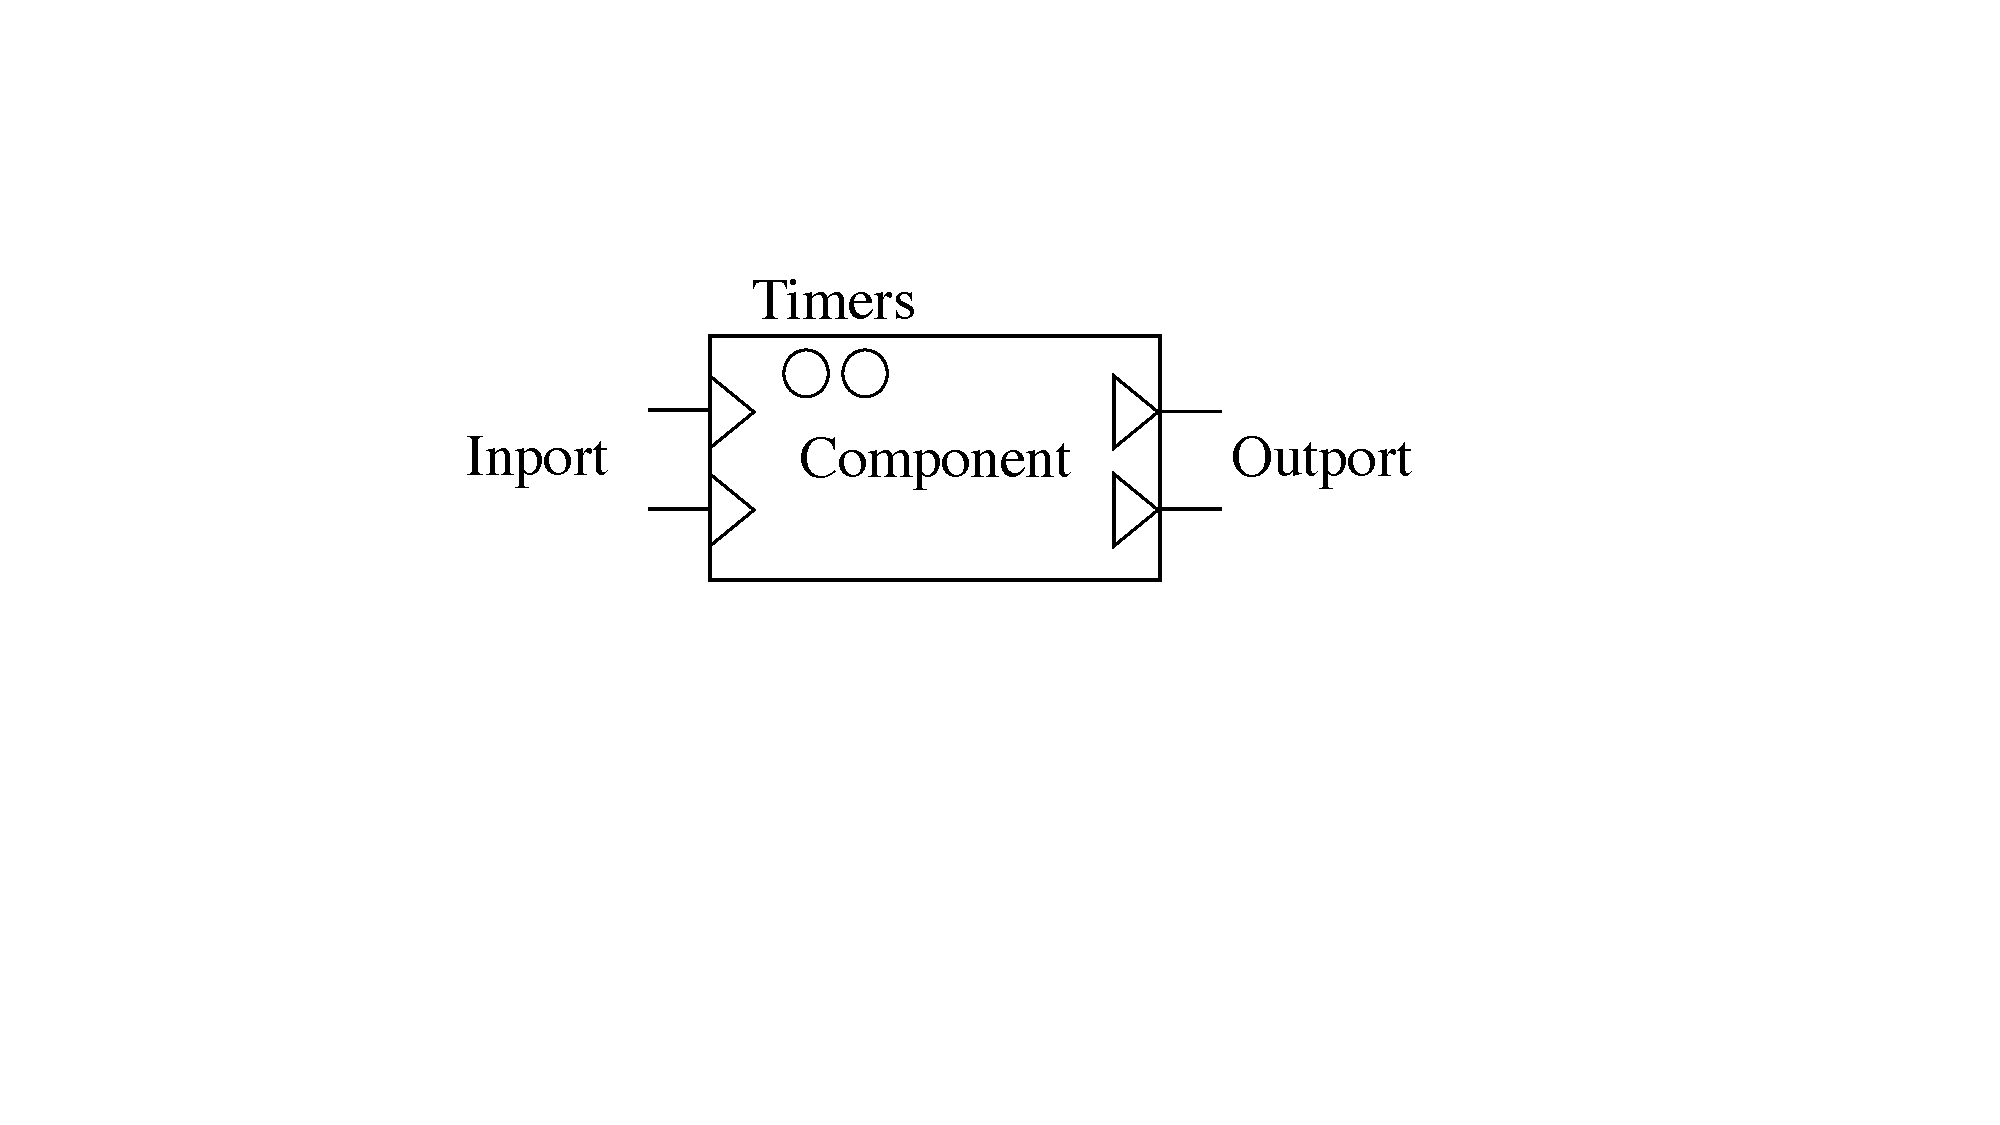
\epsfig{file=images/cost.pdf, width=7cm}
		\caption{COST component}
		\label{fig:cost}
	\end{figure}	
	
	%%%  Structure
	\subsection{Paper Structure}
	\label{section:structure}
	This documents is structured as follows: Section \ref{section:system_model} describes the system model. Then, Section \ref{section:mac_features} defines the implementation of MAC functionalities considered so far.
	
%%%%%%%%%%%%%%%
% 2. SYSTEM MODEL
%%%%%%%%%%%%%%%
\section{System Model}
\label{section:system_model}
One of the main tasks regarding the implementation of Komondor is the definition of the system model, which lays the foundations of the simulator. In this Section we describe the models defined for simulating the different communication aspects that wireless device implement.
	
	%%% Channel Modeling
	\subsection{Channel Modeling}
	Channel modeling is one of the most important parts regarding the system model, since it has direct impact on the interactions between wireless devices. For that, and in order to provide the most representative wireless environments, we implemented the following set of path-loss models, which can be further extended by any developer:
	\begin{itemize}
		\item Free Space Path Loss (FSPL): a free-space model is considered, which captures direct line-of-sight and ignores shadowing effects. The experienced loss of power during a transmission that assumes this model is given by:
		\begin{equation}
			\text{FSPL} = 20 \log_{10}(d) + 20 \log_{10}(f) + 20 \log_{10}(\frac{4\pi}{c}) - G_t - G_r,
			\nonumber
		\end{equation}
		where $d$ is the distance between the transmitter and the receiver, $f$ is the frequency used in GHz, $c$ is the light speed in $m/s$, and $G_t$ and $G_r$ are the gains in dB at the transmitter and receiver, respectively.
		\item Okumura-Hata model \cite{hata1980empirical}: this well-known model was conceived for predicting the path-loss of cellular transmissions in outside urban and rural environments. Our main concern is related to dense urban areas, so the loss, $L_U$, that is considered to be experienced during a transmission is given by: 
		\begin{equation}
		\begin{aligned}
			L_U =  &69.55 + 22.16 \log_{10}(f) - 13.82 \log_{10} (h_B) + (44.9 - 6.55 \log_{10}(h_B)) \log_{10}(d) - \\ 
			& 3.2 \log_{10}(11.7554 h_M)^2 - 4.97,
		\end{aligned}
		\nonumber
		\end{equation}
		where $f$ is the center frequency in MHz, $h_B$ is the height of the transmitter antenna (fixed to 10 m), $d$ is the distance between the transmitter's and the receiver in meters, and $h_M$ is the height of the receiver's antenna (fixed to 10 m).
		\item Indoor model: this model represents a simple indoor scenario, which is useful to simulate typical scenarios such as flats, schools or restaurants. According to this model, the losses $L_{indoor}$ experienced between a packet transmission are:		
		\begin{equation}
			L_{indoor} = 5 + 10 \alpha \log_{10}(d) + h_S + (\frac{d}{f_w}) h_O,
			\nonumber
		\end{equation}
		where $\alpha$ is a constant that depends on the propagation model (set to 4.4), $d$ is the distance in meters between the transmitter and the receiver, $h_S$ is the shadowing factor, $f_w$ is the frequency of walls (set to one wall each 5 meters), and $h_{O}$ is the obstacles factor.
		\item Indoor model with random channel effects: we consider the same model as before, but now we introduce random variables to determine the shadowing and obstacles effects in the power losses.
		\item Residential path-loss model IEEE 802.11ax: such model is included in the 11ax amendment, and captures the path-loss effects of a typical apartments building. The losses experienced between a packet transmission are:
		\begin{equation}
			\nonumber
		\end{equation}
	\end{itemize}
	
	In addition to path-loss types, we also defined different co-channel interference models to capture several kinds of interactions between devices:
	\begin{itemize}
		\item Without adjacent interference: no power is leaked to adjacent channels.
		\item Full channel interference: power from other channels i leaked, so that a 20 dBr decrease is noticed for each channel distance. For instance, the power that channel 1 leaks into channel 3 is the actual power in channel 1 minus 40 dBr. 
		\item Limited adjacent interference: in this case, only immediate adjacent channels leak power to the target one.
	\end{itemize}
	
	An example of channels overlapping is shown in Figure \ref{fig:cochannel_interference}.
	\begin{figure}[h!]
		\centering
		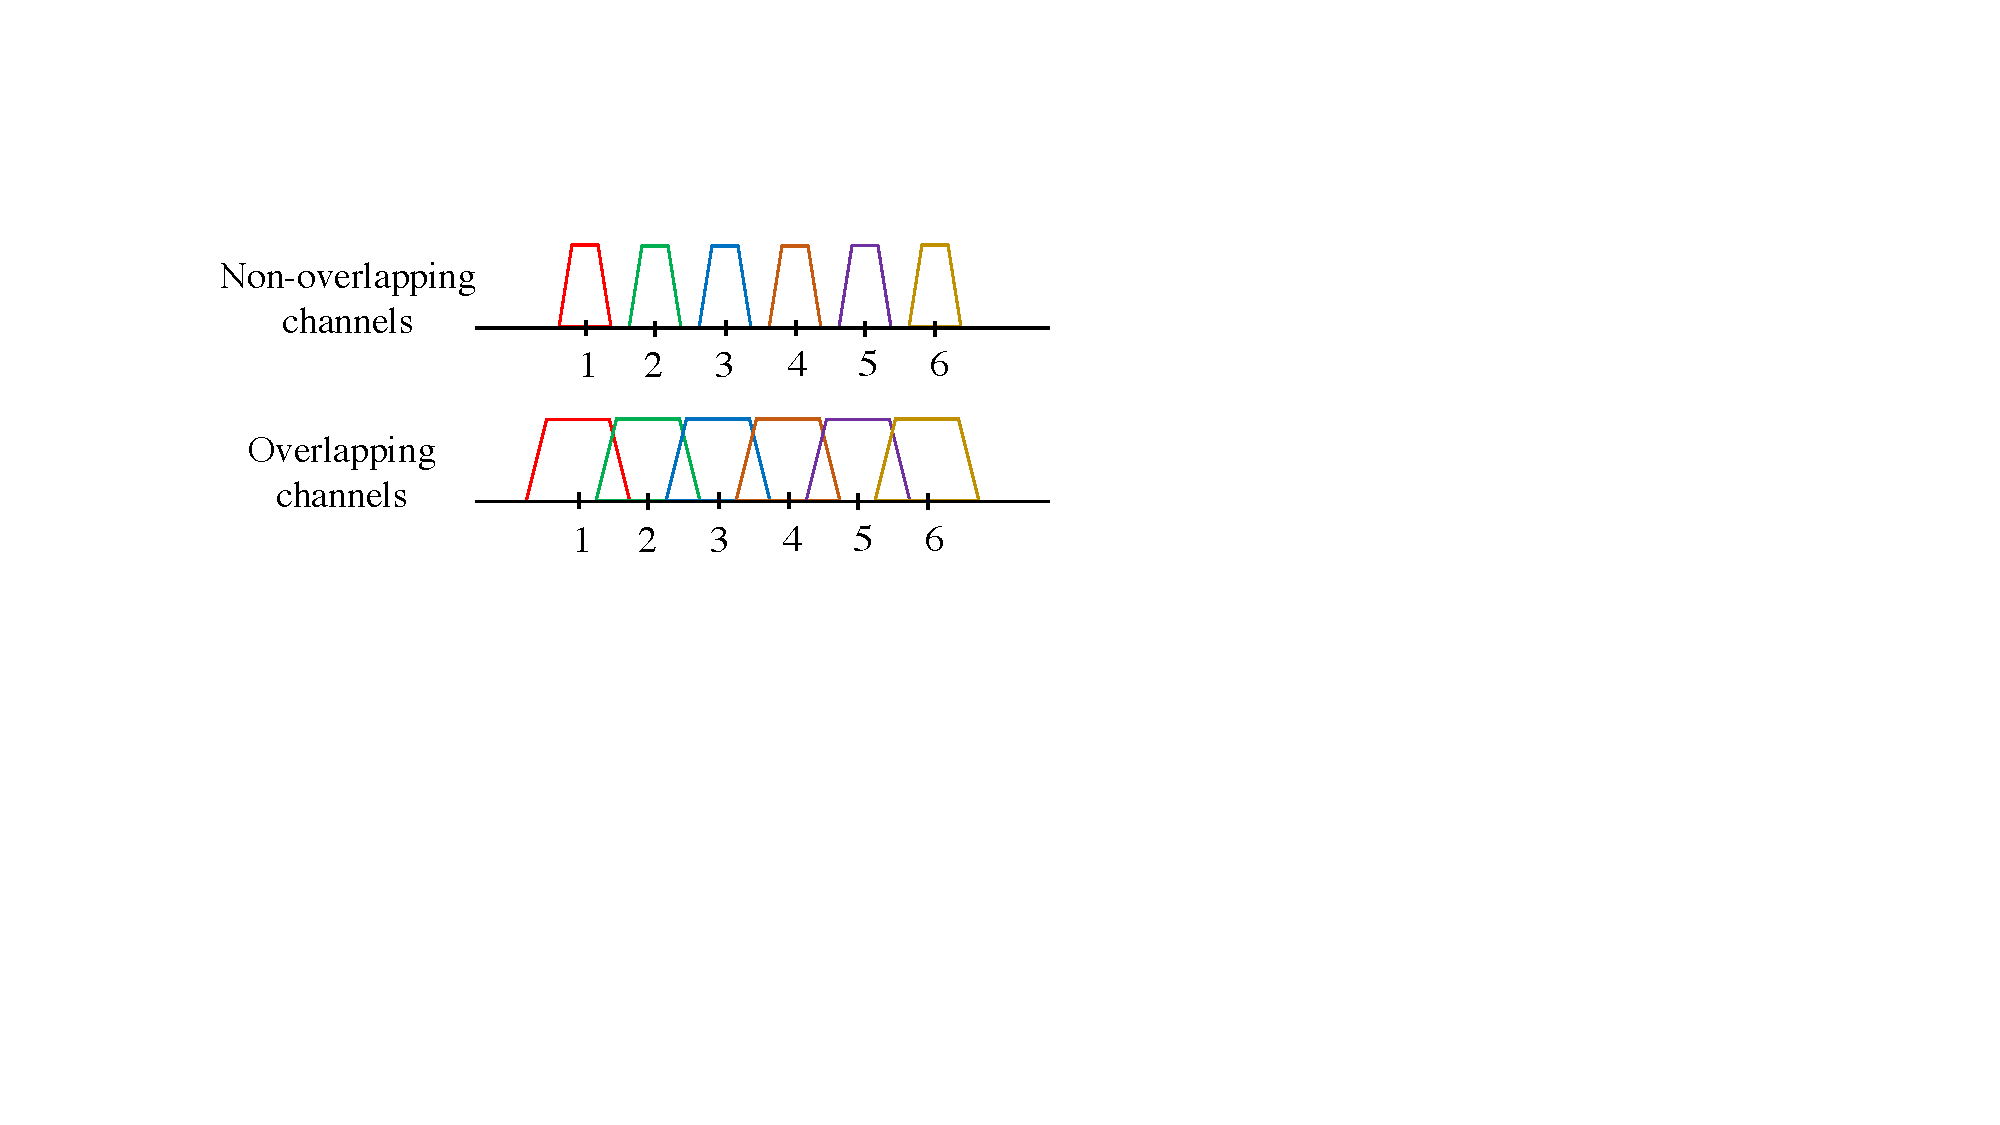
\epsfig{file=images/cochannel_interference.pdf, width=9cm}
		\caption{Channel models with and without adjacent interference}
		\label{fig:cochannel_interference}
	\end{figure}	
		
	Finally, regarding the channel model, it is important to remark that the incoming power is assumed to be the same during the entire transmission. This relaxation allows us to easily determine whenever the channel of interest is busy or not. A direct implication of it affects to path-loss models used, as well as some of them assume random variations of the medium, preventing to obtain the same result with different power received calculations (so far, power received is added and subtracted when the node accesses and leaves the channel, respectively). Thus, for each node we store its incoming power (which is computed only once) for subtracting it at the end of its transmission. 
	
	%%% Traffic modeling
	\subsection{Traffic Modeling}
	\label{section:traffic_modelling}
	Traffic modeling refers to the capacity of generating data in higher transmission layers. So far, Komondor only considers downlink traffic, so that data transmissions are initiated by APs. Regarding traffic generation, we have considered three different models:
	\begin{itemize}
		\item Full buffer: transmitters are in a permanent saturation regime, so that they always have packets to be sent.
		\item Poisson: packets are generated according to a Poisson distribution, so that the time between packets $\Delta_p$ is determined by the packet generation rate $\lambda$, and is given by $\Delta_{\rm p} = e^{\frac{1}{\lambda}}$
		\item Deterministic: packets are generated at fixed time intervals, $\Delta_d$, given by the packet generation rate, $\Delta_{\rm d} = 1/\lambda$.
	\end{itemize}

	Figure \ref{fig:traffic_models} illustrates the aforementioned traffic models. 
	\begin{figure}[h!]
		\centering
		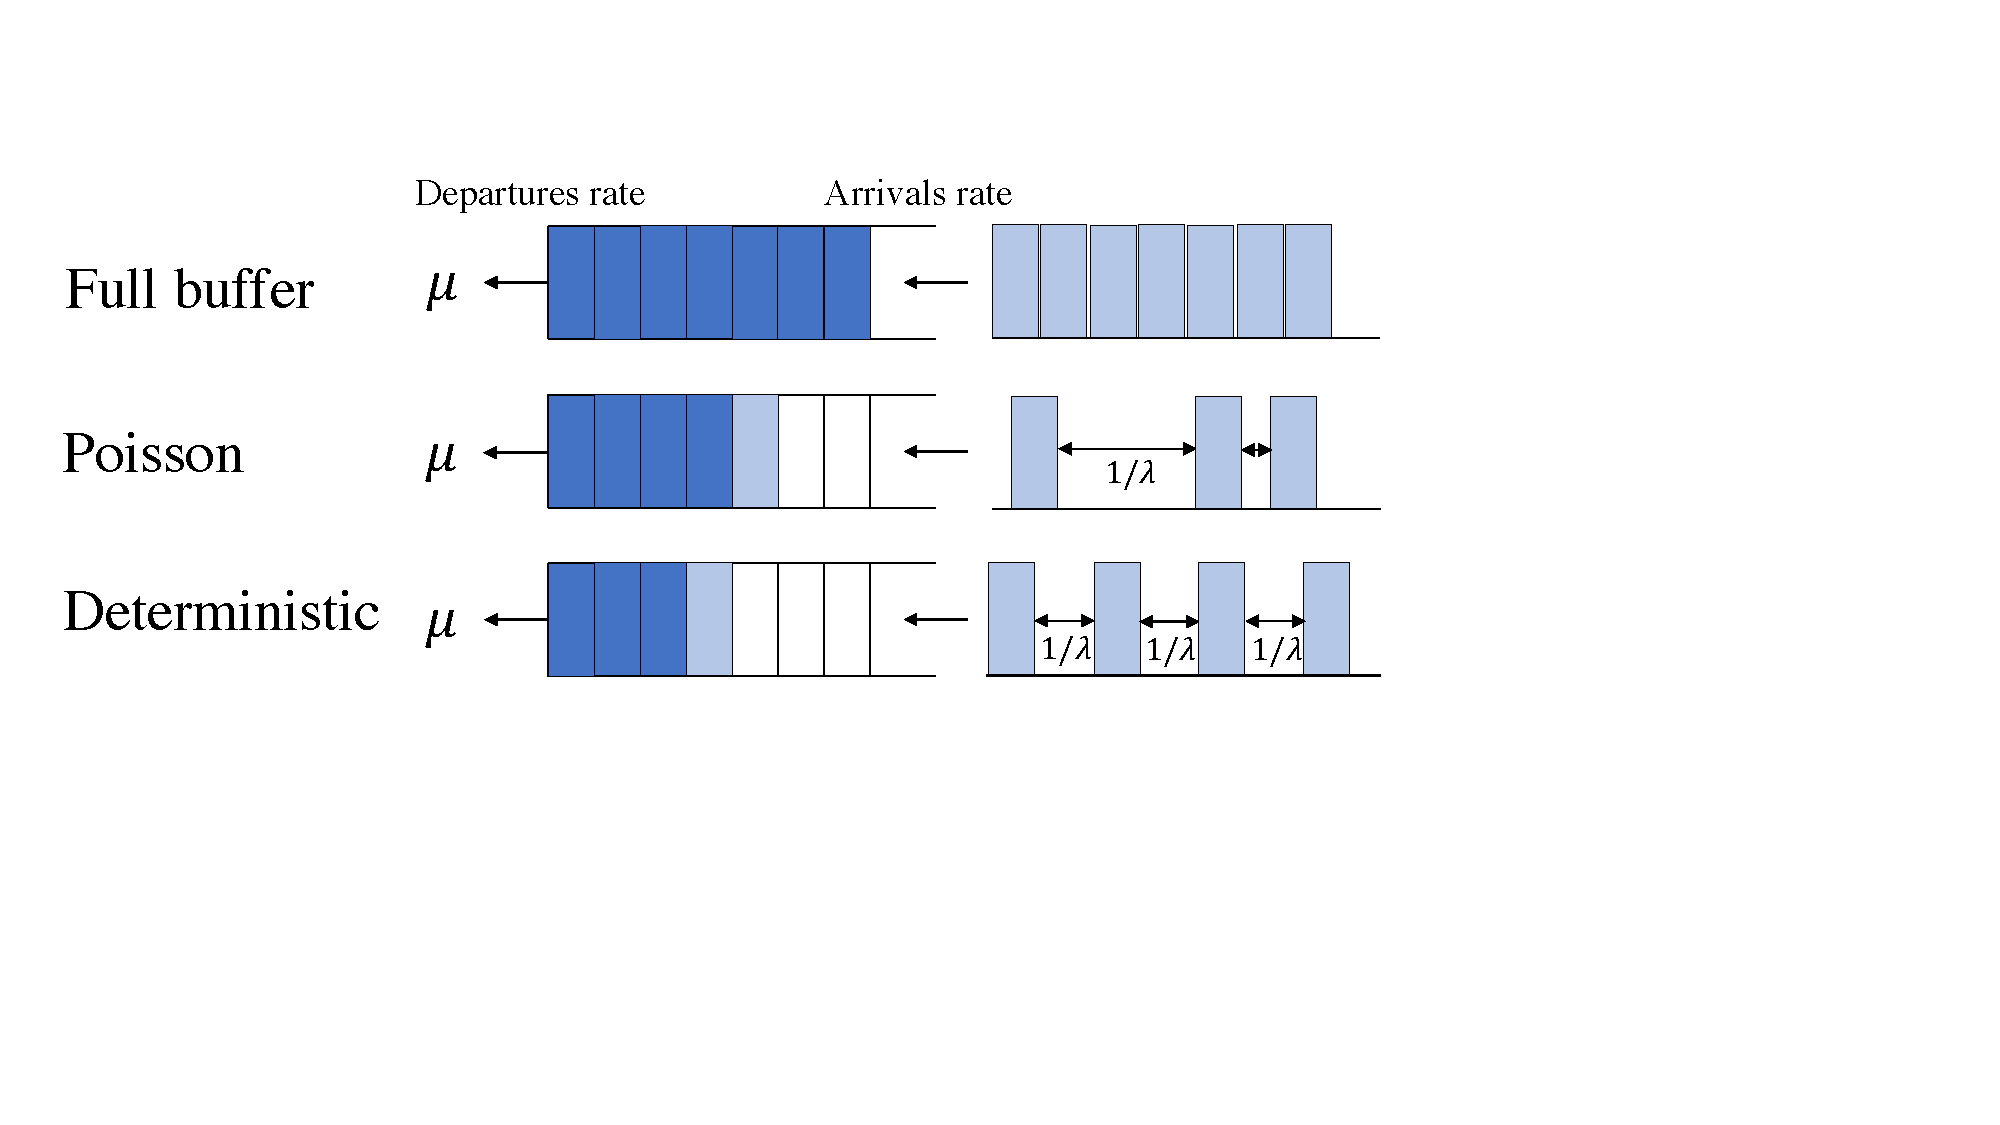
\epsfig{file=images/traffic_models.pdf, width=9cm}
		\caption{Traffic models used in Komondor}
		\label{fig:traffic_models}
	\end{figure}	
	
	%%% Data rate modeling
	\subsection{Link Modeling}
	In order to determine the data rate to be used during a given transmission, the MCS defined in the IEEE 802.11ax are considered. Komondor assumes that the MCS used between a pair of devices is determined by the SINR at the received, so that the maximum allowable MCS is used. The required SINR that corresponds to each MCS is defined in Table \ref{table:sinr_thresholds_mcs}, as well as the granted data rate for each channel width.
	% MCS IEEE 802.11ax
	\begin{table}[]
		\centering
		\resizebox{\textwidth}{!}{\begin{tabular}{|c|c|c|c|c|c|c|c|}
			\hline
			\multirow{2}{*}{\textbf{\begin{tabular}[c]{@{}c@{}}MCS \\ index\end{tabular}}} &
			\multirow{2}{*}{\textbf{\begin{tabular}[c]{@{}c@{}}SINR \\ interval (dBm)\end{tabular}}} &
			\multirow{2}{*}{\textbf{\begin{tabular}[c]{@{}c@{}}Modulation\\ type\end{tabular}}} & \multirow{2}{*}{\textbf{\begin{tabular}[c]{@{}c@{}}Coding\\ rate\end{tabular}}} & \multicolumn{4}{c|}{\textbf{Data rate (Mbps)}} \\ \cline{5-8} 
			& &  &  & \textbf{20 MHz} & \textbf{40 MHz} & \textbf{80 MHz} & \textbf{160 MHz} \\ \hline
			0 & {[}-82, -79) & BPSK & 1/2 & 4 & 8 & 17 & 34 \\ \hline
			1 & {[}-79, -77) & QPSK & 1/2 & 16 & 33 & 68 & 136 \\ \hline
			2 & {[}-77, -74) & QPSK & 3/4 & 24 & 49 & 102 & 204 \\ \hline
			3 & {[}-74, -70) & 16-QAM & 1/2 & 33 & 65 & 136 & 272 \\ \hline
			4 & {[}-70, -66) & 16-QAM & 3/4 & 49 & 98 & 204 & 408 \\ \hline
			5 & {[}-66, -65) & 64-QAM & 2/3 & 65 & 130 & 272 & 544 \\ \hline
			6 & {[}-65, -64) & 64-QAM & 3/4 & 73 & 146 & 306 & 613 \\ \hline
			7 & {[}-64, -59) & 64-QAM & 5/6 & 81 & 163 & 340 & 681 \\ \hline
			8 & {[}-59, -57) & 256-QAM & 3/4 & 98 & 195 & 408 & 817 \\ \hline
			9 & {[}-57, -54) & 256-QAM & 5/6 & 108 & 217 & 453 & 907 \\ \hline
			10 & {[}-54, -52) & 1024-QAM & 3/4 & 122 & 244 & 510 & 1021 \\ \hline
			11 & $\geq$ 52 & 1024-QAM & 5/6 & 135 & 271 & 567 & 1143 \\ \hline
		\end{tabular}}
		\caption{Data rates granted per MCS in IEEE 802.11ax. Guard Intervals (GI) of 1600 ns are only considered.}
		\label{table:sinr_thresholds_mcs}	
	\end{table}
	
	So far, link adaptation is not considered\footnote{Future work contemplates the inclusion of Minstrel as a rate adaptation scheme.}, so that the MCS to be used between each transmitter-receiver pair is negotiated at the beginning of the first transmission, and remains static during all the simulation. In practice, the highest possible modulation is computed for each number of channels used according to the power received (the transmit power is lower as the number of channels used is higher).  With that, we aim to simulate the Receiver Driver Protocol, at which few symbols are transmitted at the lowest bit-rate for all the subcarriers. Thus, according to the SINR perceived at the receiver, the MCS is chosen and communicated to the transmitter.
		
	Finally, regarding the transmission time for sending a packet, it is computed as a function of the data rate and the size of the packet to be transmitted. Packet lengths are defined according to the IEEE 802.11ax specification, which is further described in Section \ref{section:parameters}.

	%%% Collisions model
	\subsection{Collisions Modeling}
	Collisions are one of the main issues in WLANs, since they harm the experienced performance. In particular, packet losses mostly occur because of backoff collision, hidden-node effects and link asymmetries. An example of a hidden-node collision is shown in Figure \ref{fig:collisions_hidden_node}, in which nodes A and C transmit simultaneously to B, since they do not sense the other's transmission.	
	\begin{figure}
		\centering
		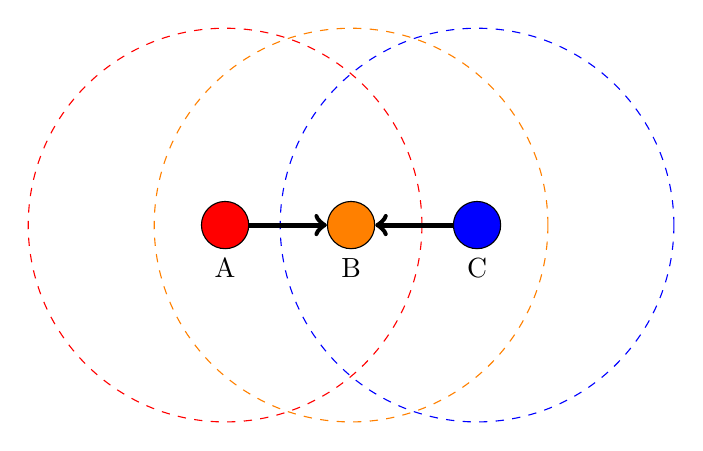
\begin{tikzpicture}
		\node at (0,0) [circle, fill=red, draw, minimum width=0.6cm,minimum height=0.6cm, label=below:$\text{A}$] (A) {};
		\node at (A) [circle,draw=red, minimum size=5cm, dashed] (Ac) {};
		\node[circle, fill=orange, draw, minimum width=0.6cm,minimum height=0.6cm, label=below:$\text{B}$] (B) [right of=A, xshift=0.6cm] {};
		\node at (B) [circle,draw=orange, minimum size=5cm, dashed] (Bc) {};
		\node[circle,draw, fill=blue, minimum width=0.6cm,minimum height=0.6cm, label=below:$\text{C}$] (C) [right of=B, xshift=0.6cm] {};
		\node at (C) [circle,draw=blue, minimum size=5cm, dashed] (Cc) {};      
		\draw [->,line width=1.8pt] (A) edge (B) (C) edge (B);
		\end{tikzpicture}
		\caption{Hidden-node cause of collision} \label{fig:collisions_hidden_node}
	\end{figure}

	In Komondor, a packet loss is considered when the ACK timeout is over. However, it is critical to identify what caused such loss, which may allow to solve the root problem. In particular, the following packet losses categories are provided:
	\begin{itemize}
		\item PACKET\_LOST\_DESTINATION\_TX: packet is discarded because the destination was already transmitting when the packet transmission was attempted.
		\item PACKET\_LOST\_LOW\_SIGNAL: the packet cannot be decoded because the signal strength is not enough (i.e., it is less than capture effect).
		\item PACKET\_LOST\_INTERFERENCE: packet is lost due to interference signals that makes the receiver not accomplish the capture effect condition.	
		\item PACKET\_LOST\_PURE\_COLLISION: packet is lost because two nodes transmit to same destination with signal strengths enough to be decoded	(the situation shown in Figure \ref{fig:collisions_hidden_node}).	
		\item PACKET\_LOST\_LOW\_SIGNAL\_AND\_RX: the destination is already receiving data when a new data transmission starts. In addition, the newest signal strength is not enough to be decoded in normal conditions.
		\item PACKET\_LOST\_RX\_IN\_NAV: packet is lost because the target node is in a NAV period (it previously decoded an RTS/CTS sequence).		
		\item PACKET\_LOST\_BO\_COLLISION: the packet is lost because a backoff collision occurred, i.e., two or more interfering devices ended their backoff simultaneously.
	\end{itemize}	
	
	Furthermore, other types of collisions that are uncontrolled may occur. For instance, when applying Channel Bonding, the situation depicted in Figure \ref{fig:boat1} may occur.
	\begin{figure}[h!]
		\centering
		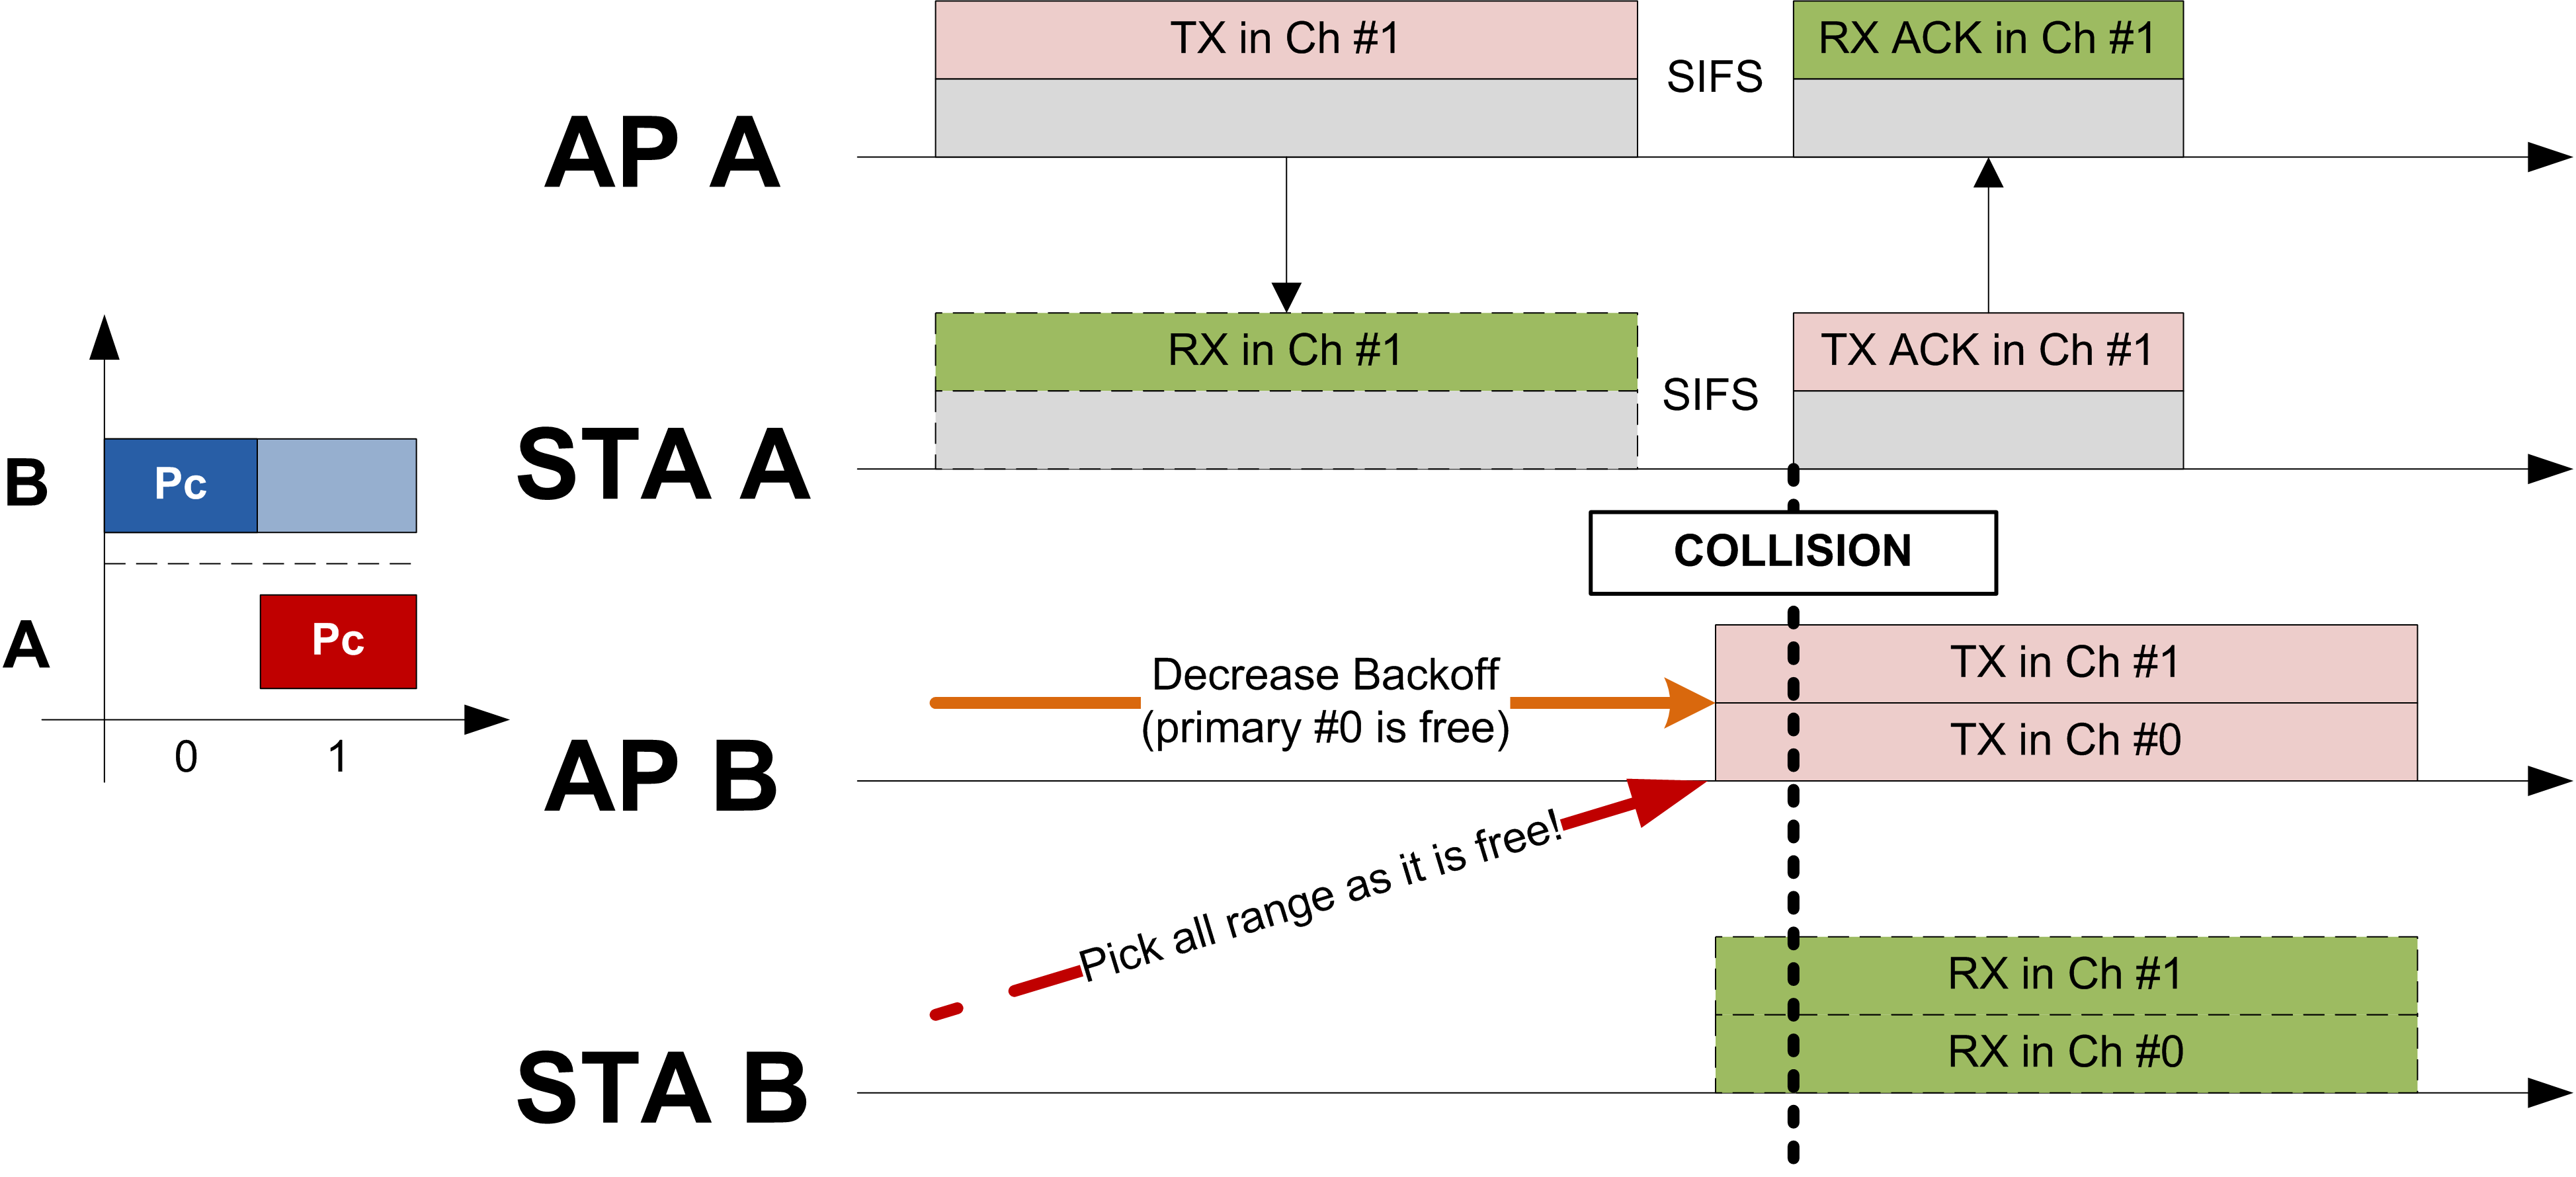
\includegraphics[scale=0.7]{images/ACK_issue.png}
		\caption{Weird case when collisions occur due to last transmitting AP checks the channel right in the SIFS period of other WLAN and picks a range affecting the previous transmission.}
		\label{fig:boat1}
	\end{figure}

%%%%%%%%%%%%%%%
% MAC FEATURES
%%%%%%%%%%%%%%%
\section{MAC Features}
\label{section:mac_features}
In this Section we provide an overview of the main MAC layer features included in Komondor, as well as a glimpse on their practical implementation.
	
	%%% Channel Access
	\subsection{Channel Access}
	\label{section:channel_access}
	When an AP has a packet to be sent, it implements Carrier Sense Multiple Access with Collision Avoidance (CSMA/CA) to access the medium, which makes use of the Distribution Coordination Function (DCF). With that, transmissions are carried out if the target channel has been empty for a given Backoff (BO) time. A channel is considered to be empty if the interference in it is equal or higher than a Capture Effect (CE) threshold, which allows defining the frequency at which packet losses occur, regardless on the Modulation Coding Scheme used.
		
		% CE
		\subsubsection{Capture Effect}
		\label{section:capture_effect}
		In order to perform transmissions through the radio link, the receiver must perceive that the desired signal strength is bigger than a CE threshold, so that the received data can be distinguished among noise and interference present in the channel. Despite there are two types of interference patterns (\emph{stronger-first} and \emph{stronger-last}), Komondor only considers data transmissions in which the target packet arrives first, just as shown in Figure \ref{fig:capture_effect}. Otherwise, when a second data packet arrives in the middle of a data transmission, both packets are discarded if the second signal is stronger than the first one.
		\begin{figure}[h!]
	 		\centering
	 		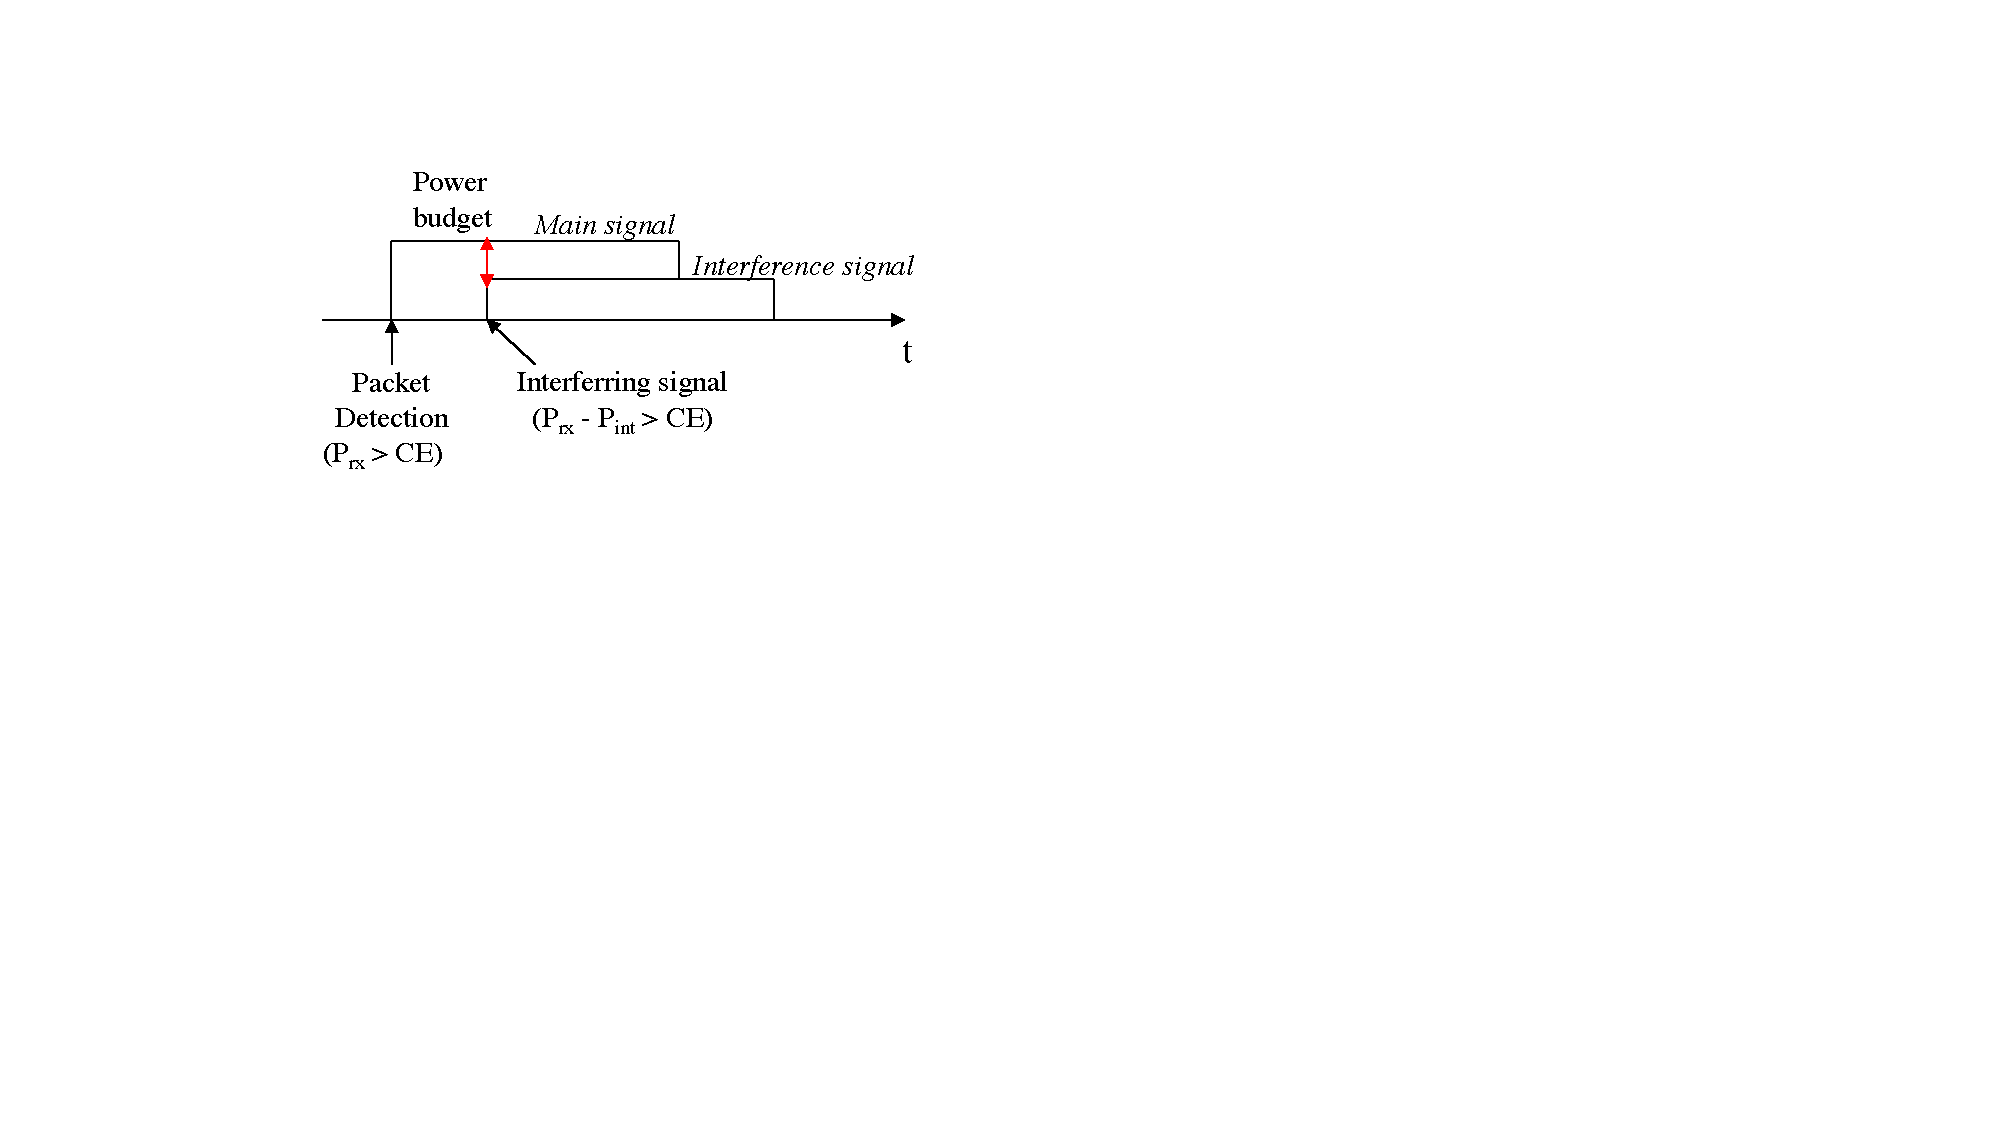
\epsfig{file=images/capture_effect, width=9cm}
	 		\caption{Stronger-First Capture Effect example}
	 		\label{fig:capture_effect}
	 	\end{figure}
 	
	 	% DCF
		\subsubsection{Distributed Coordination Function}
		\label{section:dcf}		
		As previously mentioned, the CSMA/CA operation is based on the DCF, which orchestrates channel access in a distributed manner. Roughly, transmitters (e.g., devices that have data to be transmitted) choose a random BO value, which is decremented only if the channel is sensed as idle due to the CCA condition. Otherwise, the BO is freeze and the transmission is contended. Figure \ref{fig:dcf_operation} shows an example of the DCF operation in which three nodes listen to each other in the same wireless scenario. As it is shown, STA2 wins the channel access because its BO timer is the first one to reach 0. During the packet transmission STA1 listens and does not decrease its BO. After data transmission is finished and the channel has been idle for a DIFS interval, the BO procedure is activated in all the transmitting devices.
		\begin{figure}[h!]
			\centering
			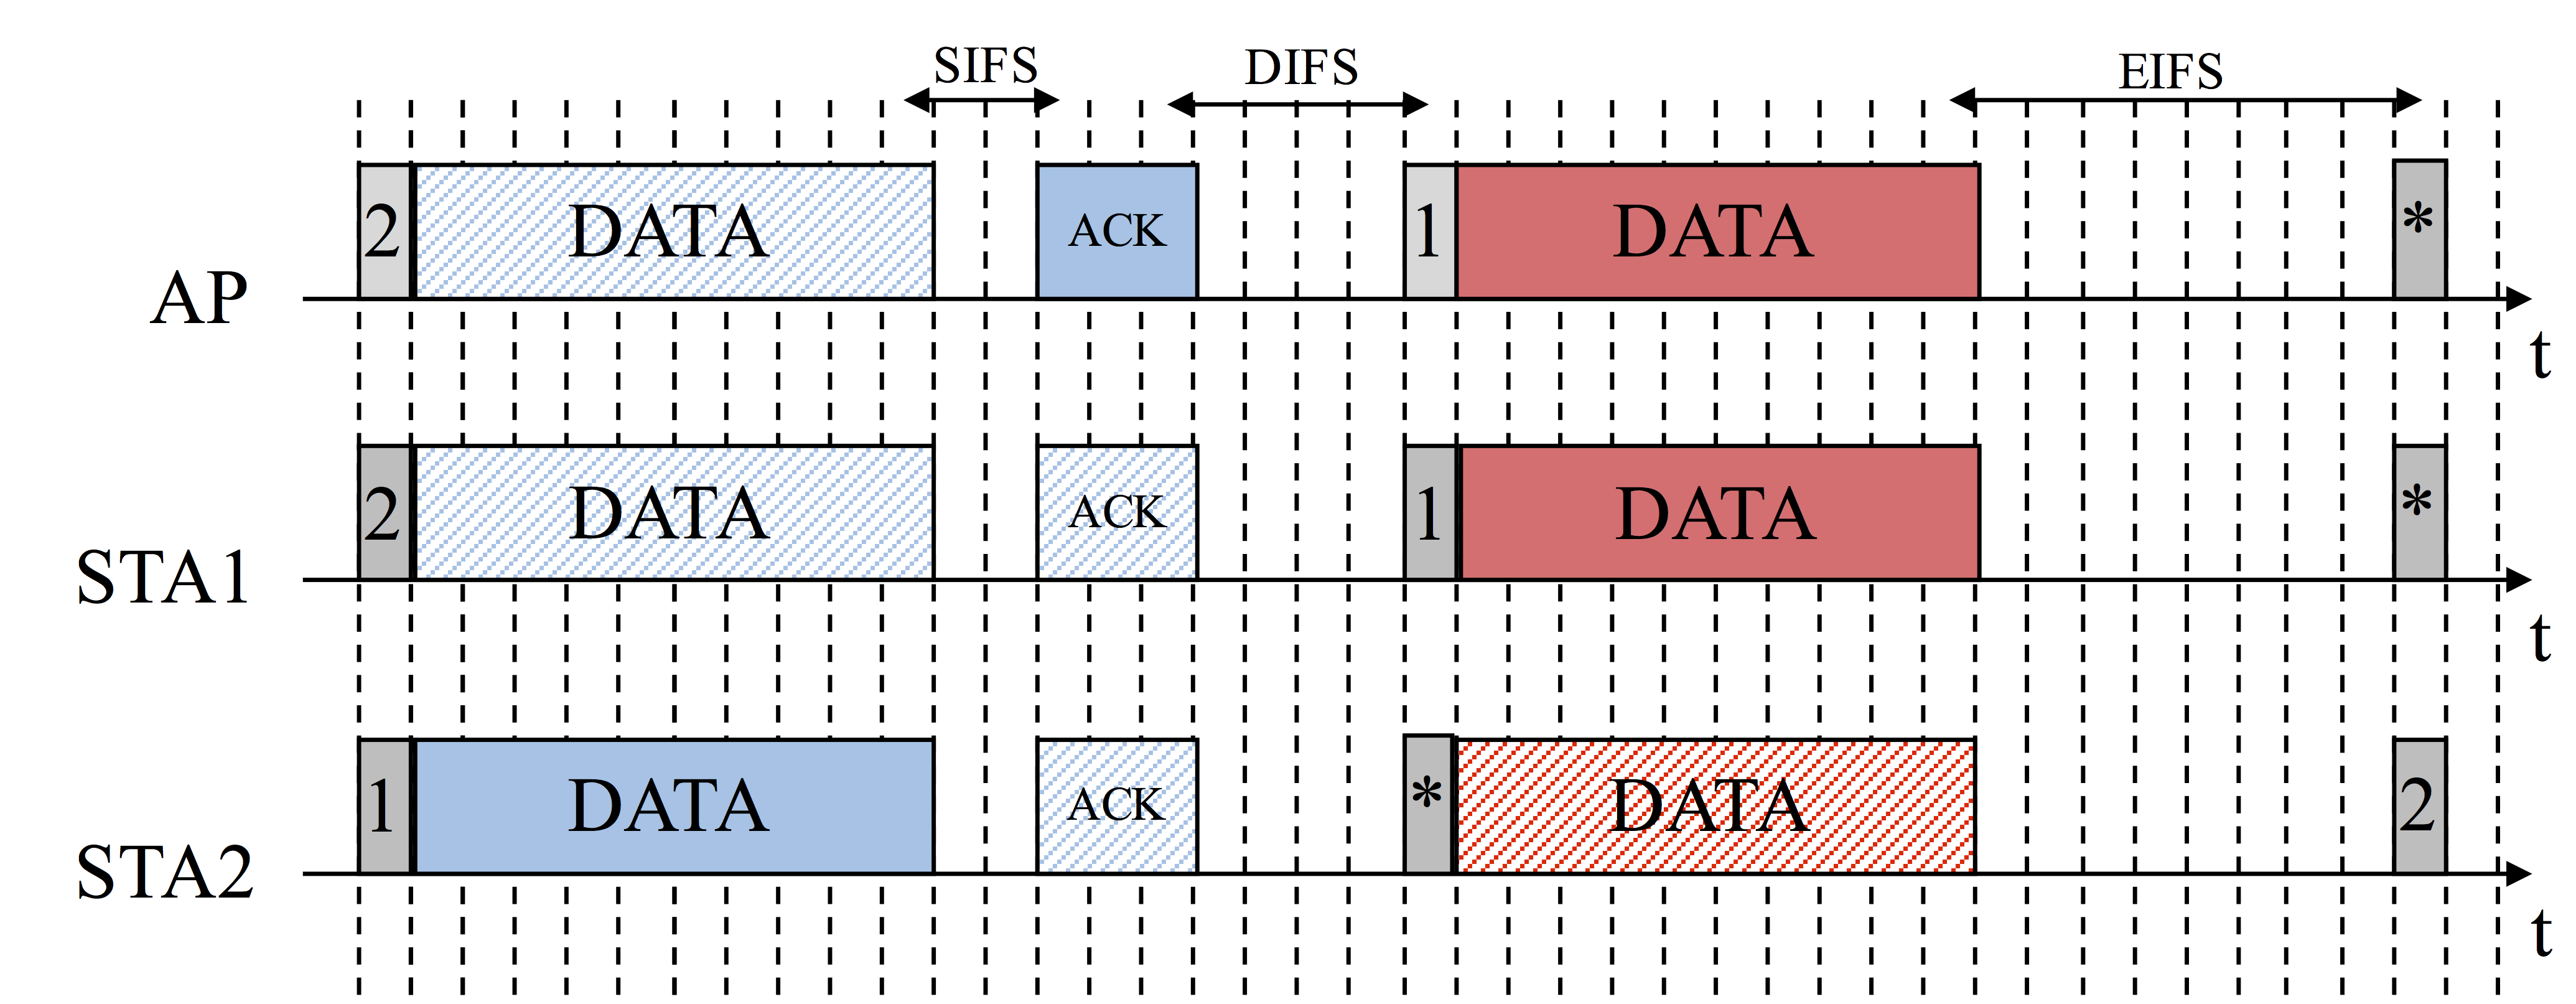
\epsfig{file=images/dcf_operation, width=12cm}
			\caption{Example of the DCF procedure}
			\label{fig:dcf_operation}
		\end{figure}
			
		The process of generating a BO before a packet transmission is determined by the Congestion Window (CW) and the generation PDF used, which has been considered to support both deterministic and exponential distributions. Komondor implements two kinds of BO pdfs to be used in different situations:
		\begin{itemize}
			\item Uniform: the BO is a number between 0 and $\text{CW}-1$, and all the values have the same probability.
			\item Exponential: instead of using an uniform distribution, we use an exponential one, so that the BO is given by a Gaussian distribution with mean $\frac{\text{CW}-1}{2}$
		\end{itemize}
				
		An important consideration with respect to discrete BO is that devices are synchronized, which allows reproducing collisions by BO that depend on the congestion window and the number of coexisting nodes.
		
		% CW Adaptation	
		\subsubsection{Contention Window Adaptation}
		\label{section:cw_adaptation}
		To complement the DCF operation, dynamic CW adaptation is considered on a per-packet basis. Optionally, one can activate CW adaptation so that the CW increases or decreases according to the situation. Given a minimum and a maximum boundaries for CW ($CW_{min}$ and $CW_{max}$, respectively), the reset operation is performed when a successful transmission is carried out. In such situation, the CW is set to $CW_{min}$. Otherwise, when packet losses occur, the CW is increased without exceeding $CW_{max}$. To do so, a counter (namely $CW_{count}$) is maintained and increased one unit each time a packet loss occurs. Then, the CW is computed as $CW = CW_{min} \times 2^{CW_{count}}$.
	
	%%% RTS/CTS
	\subsection{RTS/CTS and NAV Allocation}
	The Ready-to-Send/Clear-to-Send (RTS/CTS) mechanism is implemented in order to minimize the collisions by hidden node. Through RTS/CTS, transmitting nodes attempt to ensure that the channel would be clear during their transmissions. For that, they send control packets and wait confirmation about the clearness of the channel from the receiver's point of view. Through such packet exchange, overlapping nodes must set a virtual carrier sensing during the transmission duration, which allows reducing the collisions by hidden node. The RTS/CTS operation is exemplified in Figure \ref{fig:rts_cts_mechanism}.
	\begin{figure}[h!]
		\centering
		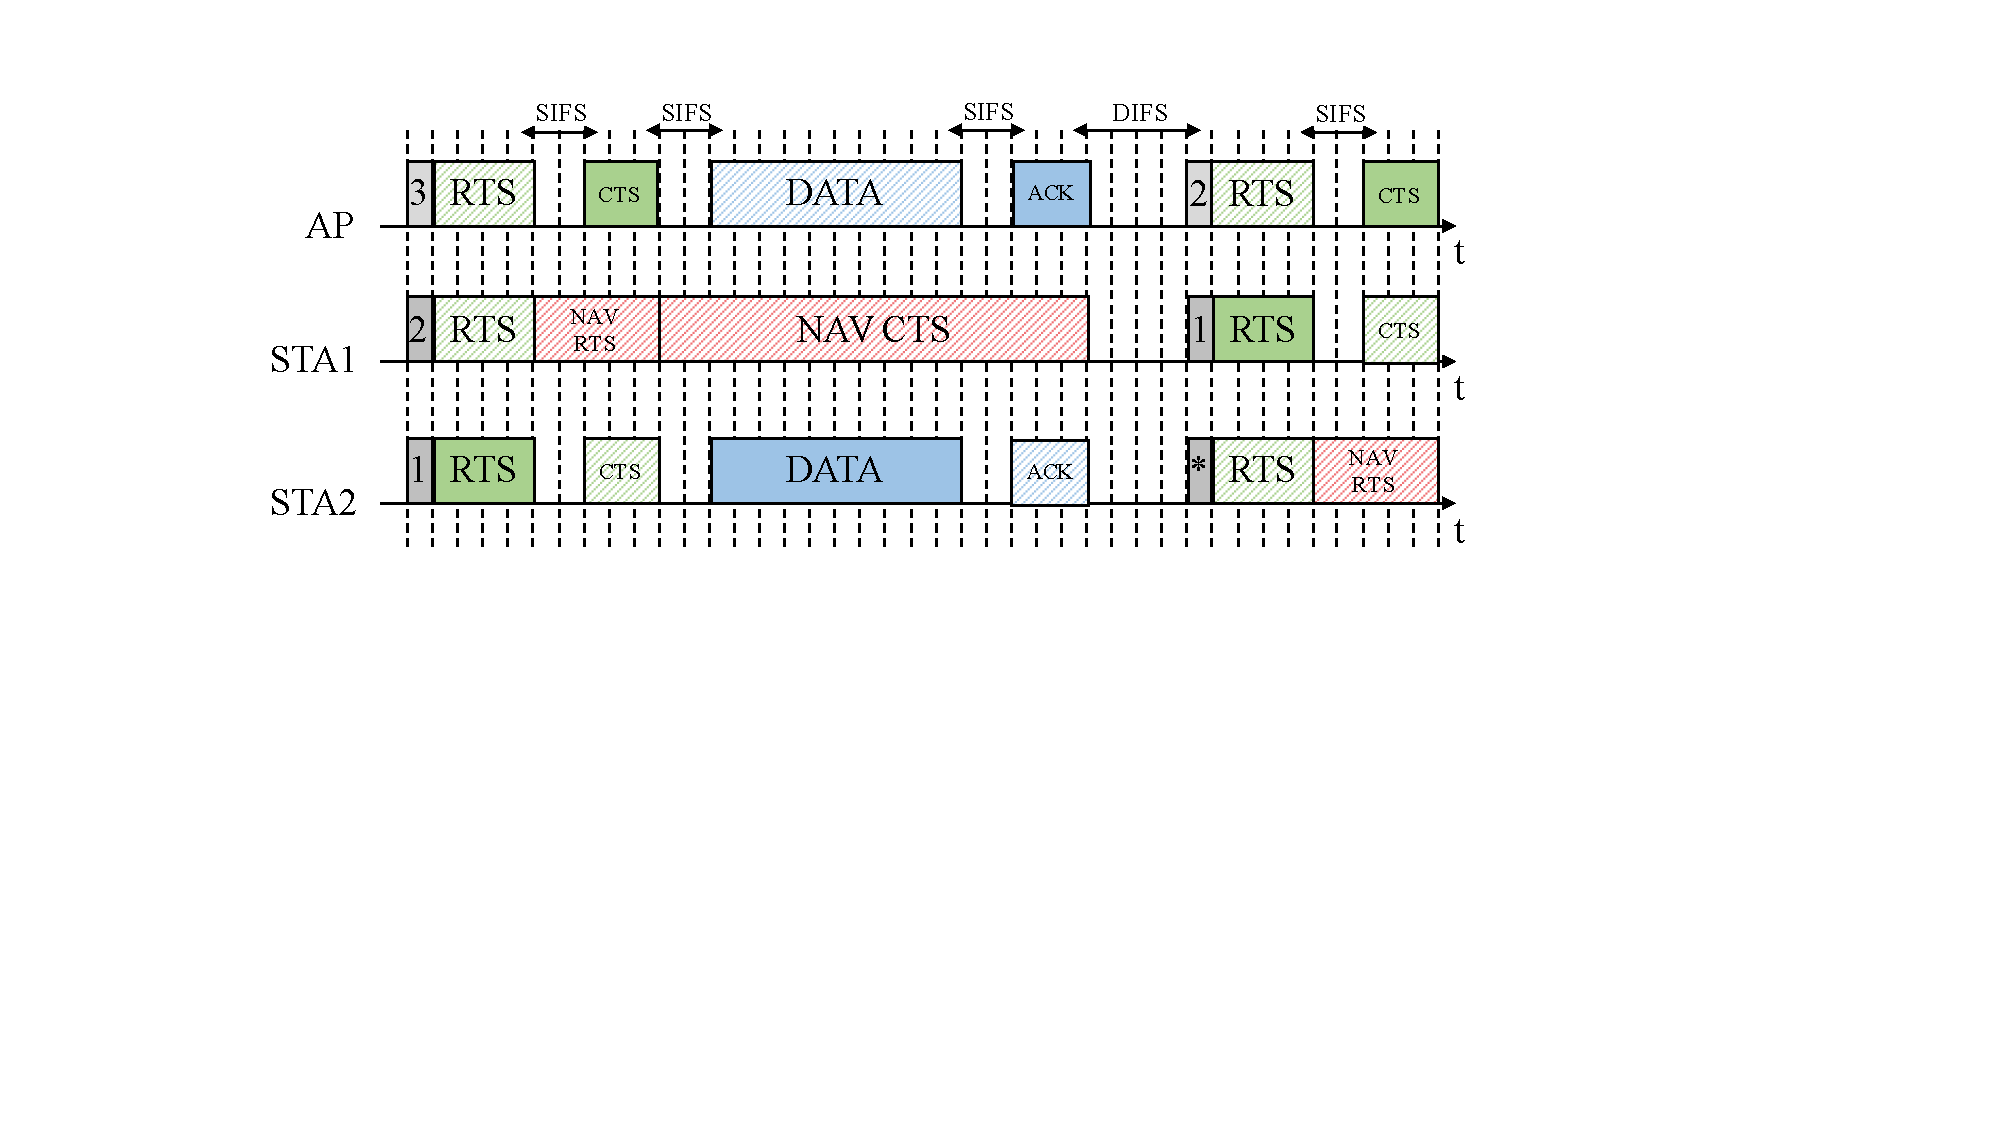
\epsfig{file=images/rts_cts_mechanism.pdf, width=12cm}
		\caption{Example of RTS/CTS implementation. The transmitter (STA2) sends an RTS packet before starting a transmission. The receiver (AP) answers with a CTS as it senses the channel free. The other coexisting devices (STA1) listen either the RTS and/or the CTS and set their NAV accordingly.}
		\label{fig:rts_cts_mechanism}
	\end{figure}	
		
	%%% Channel Bonding
	\subsection{Channel Bonding}
	\label{section:channel_bonding}
	\textcolor{red}{TO BE COMPLETED BY @SERGIO}\\
	Channel Bonding (CB) is one of the most promising techniques to enhance spectral efficiency in IEEE 802.11ax WLANs, since it aims to make the most of medium by transmitting data over several channels. For that, different CB policies are implemented in Komondor, which can be interchangeably applied by the simulated WLANs. To perform CB, one may explicitly define the available range of channels for each WLAN. Then, the following policies can be applied:
	\begin{itemize}
		\item CB disabled: the legacy operation is performed, so that only the primary channel is attempted to be accessed.
		\item Static CB: carrier sensing is performed at the primary channel. However, when attempting to transmit, all the channels within the CB range must be clear. Otherwise, a new backoff is computed.
		\begin{itemize}
		\item Aggressive SCB: 
		\item Power of 2 SCB
		\end{itemize}
		\item Dynamic:
		\begin{itemize}
			\item Aggressive DCB
			\item Power of 2 DCB\footnote{In the Matlab code, this model corresponds to the configuration \textit{onlymax = true} and \textit{selfloop = false}}: transmit in the larger channel range that is allowed by the \textit{log2} structure shown in Figure \ref{}.  
		\end{itemize}
		\item Policy-dependent:
		\begin{itemize}
			\item Sergio's PhD :D
		\end{itemize}
	\end{itemize}

	%%% Packet Aggregation
	\subsection{Packet Aggregation}
	Packet aggregation aims to reduce transmission overheads such as headers, SIFS and DIFS intervals or backoff periods. For that, it concatenates $N$ MPDUs to be sent over the same packet transmission, so that it can be acknowledged through a block ACK. Komondor allows to define the number of aggregated packets, which value remains static during the entire simulation.
	\begin{figure}[h!]
		\centering
		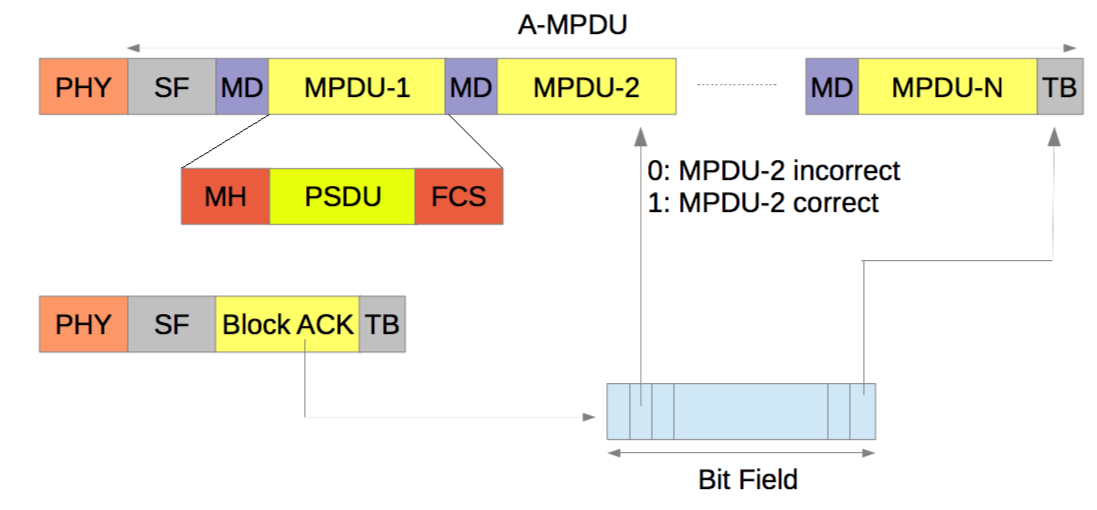
\epsfig{file=images/ampdu, width=12cm}
		\caption{Example of packet aggregation in which N MPDUs are concatenated to be sent during the same packet transmission.}
		\label{fig:ampdu}
	\end{figure}
	
%%%%%%%%%%%%%%%%
%% PHY FEATURES
%%%%%%%%%%%%%%%%
%\section{PHY Features}
%\label{section:phy_features}
%Similarly to previous Section, now we describe the PHY mechanisms implemented in Komondor.

%%%%%%%%%%%%%%%
% VALIDATIONS
%%%%%%%%%%%%%%%
\section{Komondor Main Features Validation through CTMN}
\label{section:validations}
	In this Section we focus on a set of key scenarios, which allow us to validate the Komondor's operation. For that, we use the Continuous Time Markov Networks (CTMNs) model \cite{bellalta2014throughput} for analytical comparison, which has been further extended and implemented in \cite{barrachina2017dynamic}. 

	%%% Parameters
	\subsection{IEEE 802.11ax Parameters}
	\label{section:parameters}
	Before showing the set of Komondor validations, we introduce the IEEE 802.11ax parameters that we have utilized for simulations, and which are recommended to be kept to emulate 11ax's behavior.
	
	\begin{table}[h]
		\centering
		\resizebox{\columnwidth}{!}{
			\begin{tabular}{|c|c|c|}
			\hline
			\textbf{Parameter}     & \textbf{Description}              & \textbf{Value} \\ \hline
			$\text{CW}_\text{min}$ & Min. contention window            & 16             \\ \hline
			$m$                    & Backoff stage                     & 5              \\ \hline
			CCA                    & CCA threshold                               & -82 dBm        \\ \hline
			$P_\text{tx}$          & Transmission power                & 15 dBm         \\ \hline
			$G_\text{tx}$         & Transmitting gain                 & 0 dB           \\ \hline
			$G_\text{rx}$         & Reception gain                    & 0 dB           \\ \hline
			$L_\text{data}$       & Length of a data packet at NET layer           & 12000 bits     \\ \hline
			$L_\text{BACK}$       & Length of a block ACK             & 240 bits       \\ \hline
			$L_\text{RTS}$        & Length of an RTS packet           & 160 bits       \\ \hline
			$L_\text{CTS}$        & Length of a CTS packet            & 112 bits       \\ \hline
			$n_\text{agg}$       & Number of data packets aggregated & 64             \\ \hline
			CE                     & Capture effect threshold          & 20 dB          \\ \hline
			$N$                      & Background noise level            & -95 dBm        \\ \hline
			$T_\text{slot}$       & Slot duration                     & 9 $\mu$s          \\ \hline
			SIFS                   & SIFS duration                     & 16 $\mu$s          \\ \hline
			DIFS                   & DIFS duration                     & 34 $\mu$s          \\ \hline
			PIFS                   & PIFS duration                     & 25 $\mu$s         \\ \hline
			$\eta$                 & Constant packet error rate        & 0.1           \\ \hline
			$f_c$                 & Central frequency       & 5 GHz           \\ \hline
			
			% IEEE 802.11ax
			$T_\text{ofdm}$      & Duration of OFDM symbol     & 16 $\mu$s           \\ \hline
			$T_\text{phy}$      & Duration of legacy PHY header       & 20 $\mu$s           \\ \hline
			$n_\text{ss}$               & Single user spatial streams       & 1           \\ \hline
			$T_\text{phy}^\text{HE}$      & Duration of HE header       & $(16 + n_\text{SUSS} * 16)$ $\mu$s           \\ \hline
			$L_\text{sfF}$      & Length of the MAC's service field       & 16 bits           \\ \hline
			$L_\text{del}$      & Length of the MAC's MPDU delimiter       & 32 bits           \\ \hline
			$L_\text{mac}$      & Length of the MAC header     & 272 bits           \\ \hline
			$L_\text{tail}$      & Length of the MAC's tail     & 6 bits           \\ \hline
			\end{tabular}}
			\caption{IEEE 802.11ax parameters}
			\label{table:appendix_table}
		\end{table}

	%%% Basic Scenarios
	\subsection{Basic Scenarios}
	\label{section:validations_basic_scenario}
	Through the following scenarios, we aim to validate the basic operation of Komondor, so that features such as DCF and RTS/CTS can be properly tested.	The first validation we aim to show is at a very basic scenario in which two overlapping WLANs transmit by using $a)$ the same primary channel, $b)$ different non-overlapping channels. Such scenario is depicted in Figure \ref{fig:basic_scenario_1}. Furthermore, and in order to provide a more complete validation, we test Komondor's operation in the scenario shown in Figure \ref{fig:basic_scenario_2}. The four overlapping WLANs in such scenario are intended to use $a)$ the same primary channel, $b)$ two different channels, and $c)$ four different channels. 
	\begin{figure}[h!]
	\centering
 	\begin{subfigure}[b]{0.475\textwidth}
		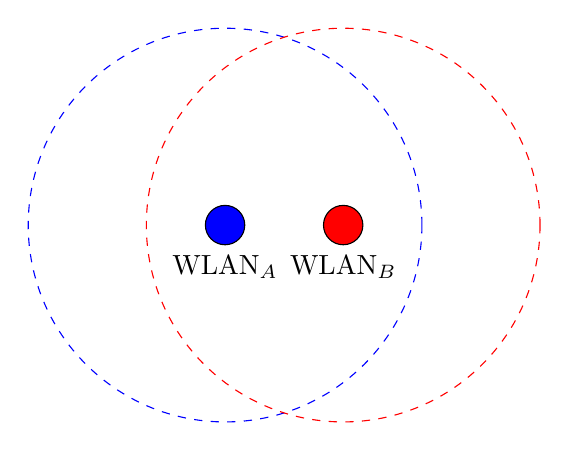
\begin{tikzpicture}
			\node at (0,0) [circle, fill=blue, draw, minimum width=0.5cm,minimum height=0.5cm, label=below:$\text{WLAN}_A$] (S1) {};
			\node at (S1) [circle,draw=blue, minimum size=5cm, dashed] (S1c) {};
			\node[circle, fill=red, draw, minimum width=0.5cm,minimum height=0.5cm, label=below:$\text{WLAN}_B$] (S2) [right of=S1, xshift=0.5cm] {};
			\node at (S2) [circle,draw=red, minimum size=5cm, dashed] (S2c) {};
		\end{tikzpicture}
		\caption{Basic scenario 1} 
		\label{fig:basic_scenario_1}
	\end{subfigure}
	\begin{subfigure}[b]{0.475\textwidth}
		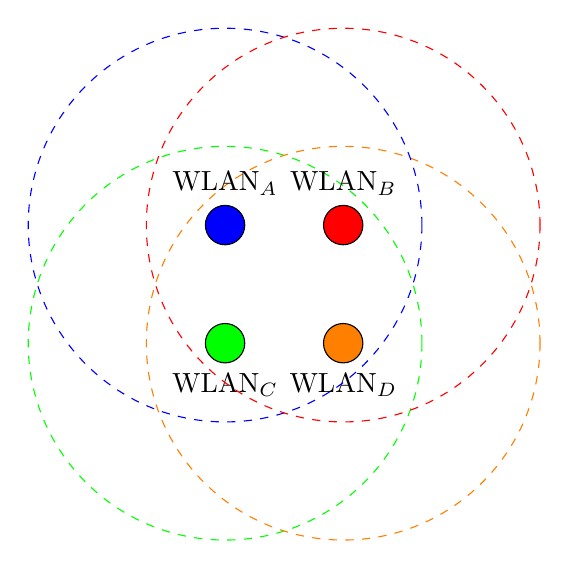
\begin{tikzpicture}
		\node at (0,0) [circle, fill=green, draw, minimum width=0.5cm,minimum height=0.5cm, label=below:$\text{WLAN}_C$] (S1) {};
		\node at (S1) [circle,draw=green, minimum size=5cm, dashed] (S1c) {};
		\node[circle, fill=orange, draw, minimum width=0.5cm,minimum height=0.5cm, label=below:$\text{WLAN}_D$] (S2) [right of=S1, xshift=0.5cm] {};
		\node at (S2) [circle,draw=orange, minimum size=5cm, dashed] (S2c) {};
		\node[circle,draw, fill=blue, minimum width=0.5cm,minimum height=0.5cm, label=above:$\text{WLAN}_A$] (S3) [above of=S1, yshift=0.5cm] {};
		\node at (S3) [circle,draw=blue, minimum size=5cm, dashed] (S3c) {};
		\node[circle,draw, fill=red, minimum width=0.5cm,minimum height=0.5cm, label=above:$\text{WLAN}_B$] (S4) [above of=S2, yshift=0.5cm] {};
		\node at (S4) [circle,draw=red, minimum size=5cm, dashed] (S4c) {};	
		\end{tikzpicture}
		\caption{Basic scenario 2}
		\label{fig:basic_scenario_2}
	\end{subfigure}
	\caption{Scenarios for basic validations}
	\label{fig:basic_scenario}
	\end{figure}

	Results from simulation in each of the basic scenarios are presented in Table \ref{table:basic_scenarios}.
	\begin{table}[h!]
		\centering
		\begin{tabular}{|c|c|c|c|c|c|c|}
			\hline
			\textbf{Scenario} & \textbf{Tool} & $\Gamma_A$ & $\Gamma_B$ & $\Gamma_C$ & $\Gamma_D$ & $\Gamma$ \\ \hline
			\multirow{2}{*}{1a} & Komondor & 51.17 & 51.12 & - & - & 102.29 \\ \cline{2-7} 
			& CTMN & 66.71 & 66.71 & - & - & 133.42 \\ \hline
			\multirow{2}{*}{1b} & Komondor & 101.66  & 101.71 & - & - & 203.37 \\ \cline{2-7} 
			& CTMN & 132.81 & 132.81 & - & - & 265.63 \\ \hline
			\multirow{2}{*}{2a} & Komondor & 12.45 & 12.50 & 12.47 & 12.49 & 49.91 \\ \cline{2-7} 
			& CTMN & 33.43 & 33.43 & 33.43 & 33.43 & e \\ \hline
			\multirow{2}{*}{2b} & Komondor & 50.99 & 50.97 & 51 & 51.02 & 203.98 \\ \cline{2-7} 
			& CTMN & 66.71 & 66.71 & 66.71 & 66.71 & 266.84 \\ \hline
			\multirow{2}{*}{2c} & Komondor & 101.19 & 101.23 & 101.18 & 101.19 & 404.78 \\ \cline{2-7} 
			& CTMN & 132.81 & 132.81 & 132.81 & 132.81 & 531.24 \\ \hline
		\end{tabular}
		\caption{Summary of the results obtained for the basic scenarios.}
		\label{table:basic_scenarios}
	\end{table}	
	
	%%% Hidden and Exposed Scenarios
	\subsection{Hidden and Exposed Node Scenarios}
	\label{section:validations_hidden_exposed}
	We start showing a hidden-node situation in which two simultaneously transmit to the their respective STAs, as shown in Figure \ref{fig:hidden_node_scenario}. Due to nodes location, transmitters (i.e., the APs) do not sense each other, so that they simultaneously transmit and generate collisions at the receivers (e.g., the STAs), which are in the middle. 
	
	Regarding the exposed node situation, we introduce the scenario depicted in Figure \ref{fig:exposed_node_scenario}, in which one of the three WLANs suffers starvation because of its location. The fact that $\text{WLAN}_A$ and $\text{WLAN}_C$ do not sense each other makes that $\text{WLAN}_B$ senses the channel busy almost all the time and lacks of opportunities for accessing to it.
	\begin{figure}[h!]
	\centering
	\begin{subfigure}[b]{0.5\textwidth}
		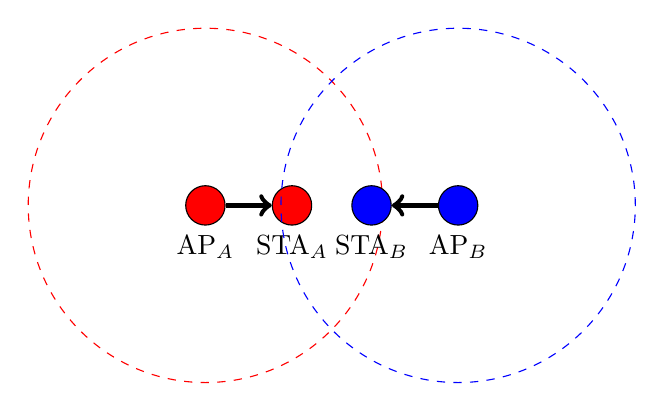
\begin{tikzpicture}
		\node at (0,0) [circle, fill=red, draw, minimum width=0.5cm,minimum height=0.5cm, label=below:$\text{AP}_A$] (A) {};
		\node at (A) [circle,draw=red, minimum size=4.5cm, dashed] (Ac) {};
		\node[circle, fill=red, draw, minimum width=0.5cm,minimum height=0.5cm, label=below:$\text{STA}_A$] (B) [right of=A, xshift=0.1cm] {};
		%\node at (B) [circle,draw=red, minimum size=3.5cm, dashed] (Bc) {};
		\node[circle,draw, fill=blue, minimum width=0.5cm,minimum height=0.5cm, label=below:$\text{STA}_B$] (C) [right of=B, xshift=0.01cm] {};
		%\node at (C) [circle,draw=blue, minimum size=3.5cm, dashed] (Cc) {};      
		\node[circle,draw, fill=blue, minimum width=0.5cm,minimum height=0.5cm, label=below:$\text{AP}_B$] (D) [right of=C, xshift=0.1cm] {};
		\node at (D) [circle,draw=blue, minimum size=4.5cm, dashed] (Cc) {};
		\draw [->,line width=1.8pt] (A) edge (B) (D) edge (C);
		\end{tikzpicture}
		\caption{Hidden-node} 
		\label{fig:hidden_node_scenario}
	\end{subfigure}
	\begin{subfigure}[b]{0.5\textwidth}
		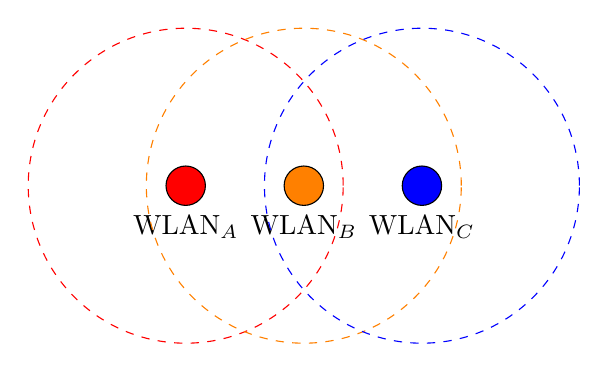
\begin{tikzpicture}
		\node at (0,0) [circle, fill=red, draw, minimum width=0.5cm,minimum height=0.5cm, label=below:$\text{WLAN}_A$] (A) {};
		\node at (A) [circle,draw=red, minimum size=4cm, dashed] (Ac) {};
		\node[circle, fill=orange, draw, minimum width=0.5cm,minimum height=0.5cm, label=below:$\text{WLAN}_B$] (B) [right of=A, xshift=0.5cm] {};
		\node at (B) [circle,draw=orange, minimum size=4cm, dashed] (Bc) {};
		\node[circle,draw, fill=blue, minimum width=0.5cm,minimum height=0.5cm, label=below:$\text{WLAN}_C$] (C) [right of=B, xshift=0.5cm] {};
		\node at (C) [circle,draw=blue, minimum size=4cm, dashed] (Cc) {};      
		\end{tikzpicture}
		\caption{Exposed-node}
		\label{fig:exposed_node_scenario}
	\end{subfigure}
	\caption{Representative scenarios of performance anomalies in WLANs} 
	\label{fig:anomalies_scenario}
	\end{figure}

	Results for both hidden and exposed scenarios are shown in Table \ref{table:hidden_exposed_scenarios}.
	% Please add the following required packages to your document preamble:
	% \usepackage{multirow}
	\begin{table}[]
		\centering
		\begin{tabular}{|c|c|c|c|c|c|c|}
			\hline
			\textbf{Scenario} & \textbf{Tool} & $\Gamma_A$ & $\Gamma_B$ & $\Gamma_C$ & $\Gamma$ & Loss rate \\ \hline
			\multirow{2}{*}{\begin{tabular}[c]{@{}c@{}}Hidden\\ node\end{tabular}} & Komondor & 0 & 0 & - & 0 & 1  \\ \cline{2-7} 
			& CTMN & 0 & 0 & - & 0 & 1 \\ \hline
			\multirow{2}{*}{\begin{tabular}[c]{@{}c@{}}Exposed\\ node\end{tabular}} & Komondor & 101.07 & 0.64 & 101.07 & 202.77 & 0.11* \\ \cline{2-7} 
			& CTMN & 131.64 & 1.19 & 131.64 & 264.47 & 0 \\ \hline
		\end{tabular}
		\caption{Summary of the results obtained for the hidden and exposed node scenarios. *A constant packet loss rate of 0.1 is set to simulate losses when using an acceptable MCS.}
		\label{table:hidden_exposed_scenarios}
	\end{table}	

	%%% Channel Bonding Scenarios
	\subsection{Channel Bonding Scenarios}
	\label{section:validations_channel_bonding}
	Finally, in order to validate the most important technique included in the first version of the Komondor simulator, we now propose a set of scenarios in which CB is applied. For that, we use the same scenario as shown in Figure \ref{fig:basic_scenario_2}, which allows us to devise several combinations regarding channel allocation. Such combinations are illustrated in Figure \ref{fig:channel_allocation_3to6}.	
	
	% Figure scenarios CB
	\begin{figure}[h]
	\centering
	  \begin{subfigure}[b]{0.475\textwidth}
	    \centering
	    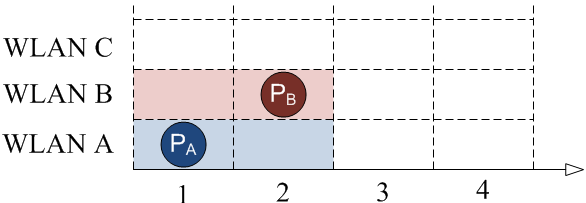
\includegraphics[width=\textwidth]{images/channel_bonding_scenario1.png}
	    \caption[]%
	    {{\small Scenario 1}}    
	    \label{fig:channel_bonding_scenario1}
	  \end{subfigure}
	  \hfill
	  \begin{subfigure}[b]{0.475\textwidth}  
	    \centering 
	    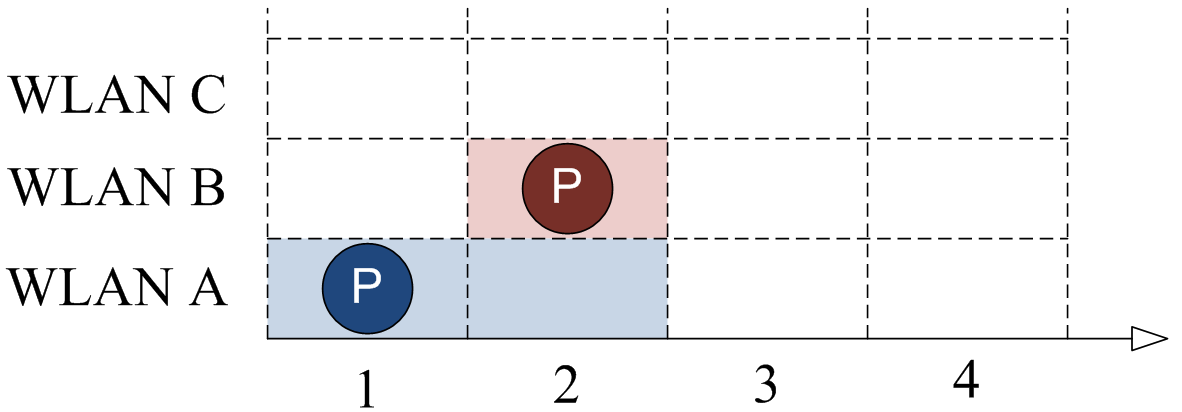
\includegraphics[width=\textwidth]{images/channel_bonding_scenario2.png}
	    \caption[]%
	    {{\small Scenario 2}}
	    \label{fig:channel_bonding_scenario2}
	  \end{subfigure}
	    \begin{subfigure}[b]{0.475\textwidth}
	    \centering
	    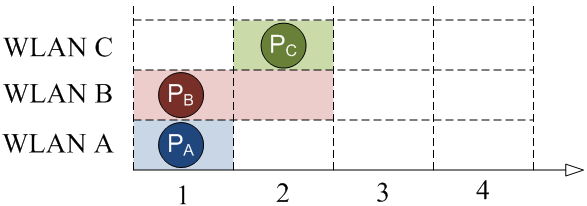
\includegraphics[width=\textwidth]{images/channel_bonding_scenario3.png}
	    \caption[]%
	    {{\small Scenario 3}}    
	    \label{fig:channel_bonding_scenario3}
	  \end{subfigure}
	  \hfill
	  \begin{subfigure}[b]{0.475\textwidth}  
	    \centering 
	    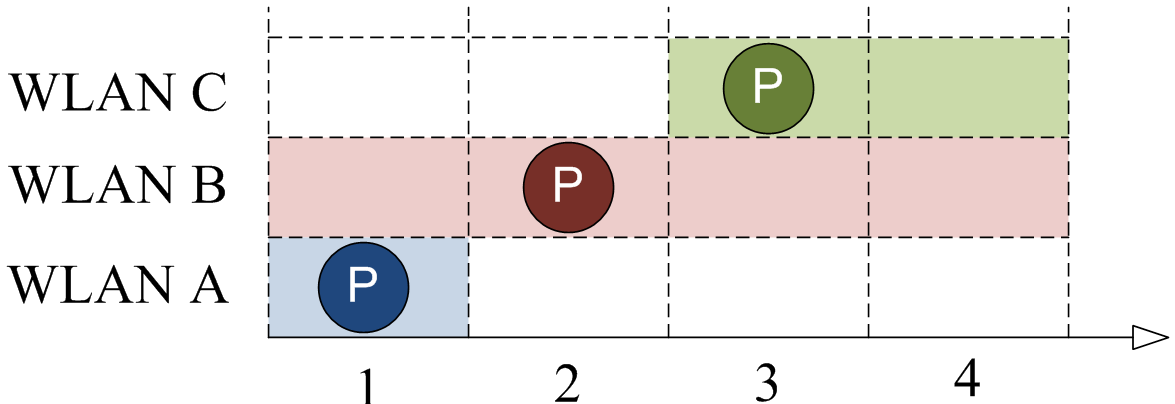
\includegraphics[width=\textwidth]{images/channel_bonding_scenario4.png}
	    \caption[]%
	    {{\small Scenario 4}}    
	    \label{fig:channel_bonding_scenario4}
	  \end{subfigure}
	  \vskip\baselineskip
	  \begin{subfigure}[b]{0.475\textwidth}   		
	    \centering 
	    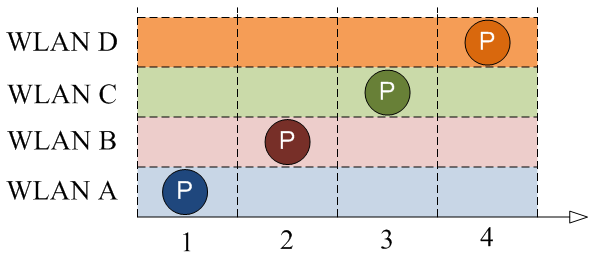
\includegraphics[width=\textwidth]{images/channel_bonding_scenario5.png}
	    \caption[]%
	    {{\small Scenario 5}}    
	    \label{fig:channel_bonding_scenario5}
	  \end{subfigure}
	  \quad
	  \begin{subfigure}[b]{0.475\textwidth}   
	    \centering 
	    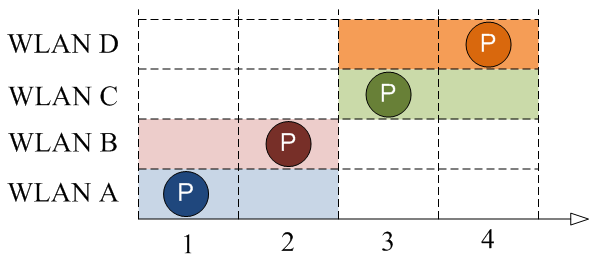
\includegraphics[width=\textwidth]{images/channel_bonding_scenario6.png}
	    \caption[]%
	    {{\small Scenario 6}}    
	    \label{fig:channel_bonding_scenario6}
	  \end{subfigure}
	  \begin{subfigure}[b]{0.475\textwidth}   		
	    \centering 
	    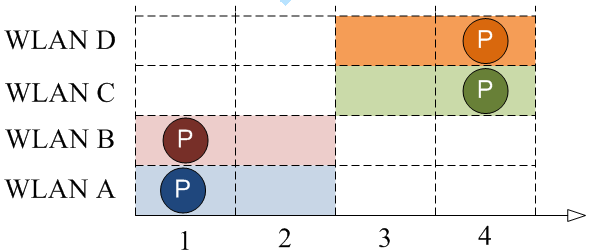
\includegraphics[width=\textwidth]{images/channel_bonding_scenario7.png}
	    \caption[]%
	    {{\small Scenario 7}}    
	    \label{fig:channel_bonding_scenario7}
	  \end{subfigure}
	  \quad
	  \begin{subfigure}[b]{0.475\textwidth}   
	    \centering 
	    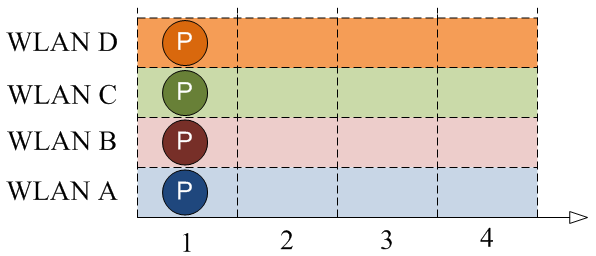
\includegraphics[width=\textwidth]{images/channel_bonding_scenario8.png}
	    \caption[]%
	    {{\small Scenario 8}}    
	    \label{fig:channel_bonding_scenario8}
	  \end{subfigure}
	\caption[Channel allocations]
	{\small Channel allocations of the different scenarios.} 
	\label{fig:channel_allocation_3to6}
	\end{figure}
	
	% Table results CB
	\begin{table}[h!]
		\centering
		\begin{tabular}{|c|c|c|c|c|c|c|c|}
		\hline
		\textbf{Scenario}                           & \textbf{States}                              & \textbf{Tool} & $\Gamma_A$ & $\Gamma_B$ & $\Gamma_C$ & $\Gamma_D$ & $\Gamma$   \\ \hline
		                                            &                                              & ACK       & 57.1418    & 57.2815    & -          & -          & 114.4234   \\ \cline{3-8} 
		\multirow{-2}{*}{1}                         & \multirow{-2}{*}{3}                          & CTMN          & 57.6166    & 57.6166    & -          & -          & 115.2331   \\ \hline
		                                            &                                              & ACK       & 62.5831    & 61.3054   & -          & -          & 123.8886   \\ \cline{3-8} 
		\multirow{-2}{*}{2}                         & \multirow{-2}{*}{5}                          & CTMN          & 62.6145    & 61.9399    & -          & -          & 124.5544   \\ \hline
		                                            &                                              & ACK       & 31.1883    & 31.1394    & 61.7620    & -          & 124.0898   \\ \cline{3-8} 
		\multirow{-2}{*}{3}                         & \multirow{-2}{*}{7}                          & CTMN          & 31.2965    & 31.2965    & 62.1671    & -          & 124.7601   \\ \hline
		\rowcolor[HTML]{FFCCC9} 
		\cellcolor[HTML]{FFCCC9}                    & \cellcolor[HTML]{FFCCC9}                     & ACK       & XXX    & XXX  & XXX   & -          & XXX \\ \cline{3-8} 
		\rowcolor[HTML]{FFCCC9} 
		\multirow{-2}{*}{\cellcolor[HTML]{FFCCC9}4} & \multirow{-2}{*}{\cellcolor[HTML]{FFCCC9}13} & CTMN          & 61.9390    & 63.1841    & 113.4185   & -          & 238.5416   \\ \hline
		                                            &                                              & ACK       & 40.8806   & 40.8506    & 40.7439    & 40.7498    & 163.2251   \\ \cline{3-8} 
		\multirow{-2}{*}{5}                         & \multirow{-2}{*}{5}                          & CTMN          & 41.2737    & 41.2737    & 41.2737    & 41.2737    & 165.0947   \\ \hline
		                                            &                                              & ACK       & XXX    &XXX    & XXX    & XXX    & XXX   \\ \cline{3-8} 
		\multirow{-2}{*}{6}                         & \multirow{-2}{*}{9}                          & CTMN          & 57.6166    & 57.6166    & 57.6166    & 57.6166    & 230.4663   \\ \hline
		                                            &                                              & ACK       & XXX    & XXX    & XXX    & XXX    & XXX   \\ \cline{3-8} 
		\multirow{-2}{*}{7}                         & \multirow{-2}{*}{9}                          & CTMN          & 57.6166    & 57.6166    & 57.6166    & 57.6166    & 230.4663   \\ \hline
		                                            &                                              & ACK       & XXX   & XXX    &XXX1    & XXX   &XXX   \\ \cline{3-8} 
		\multirow{-2}{*}{8}                         & \multirow{-2}{*}{5}                          & CTMN          & 41.2737    & 41.2737    & 41.2737    & 41.2737    & 165.0947   \\ \hline
		\end{tabular}
		\caption{Summary of the results obtained for the \textit{log2} DCB scenarios with ACK and WLANs implemented. Simulation time is 10,000 seconds.}
		\label{table:scenario_4wlans}
	\end{table}
	
%%%%%%%%%%%%%%%
% TUTORIAL
%%%%%%%%%%%%%%%
\section{Tutorial and Development Notes}
\label{section:tutorial_and_development_notes}
	In this Section we provide a brief tutorial to encourage researchers and other practitioners to use the Komondor simulation for their experiments, and even to participate in the project. 
	%%% Brief tutorial
	\subsection{Brief Tutorial}
	\label{section:brief_tutorial}
		Komondor is composed by several modules that allow performing simulations with a high degree of freedom. In this Section we provide some details on the most important modules, as well as on its practical execution. Figure \ref{fig:komondor_flowchart} summarizes the main operations carried out by Komondor.
		\begin{figure}[h!]
			\centering
			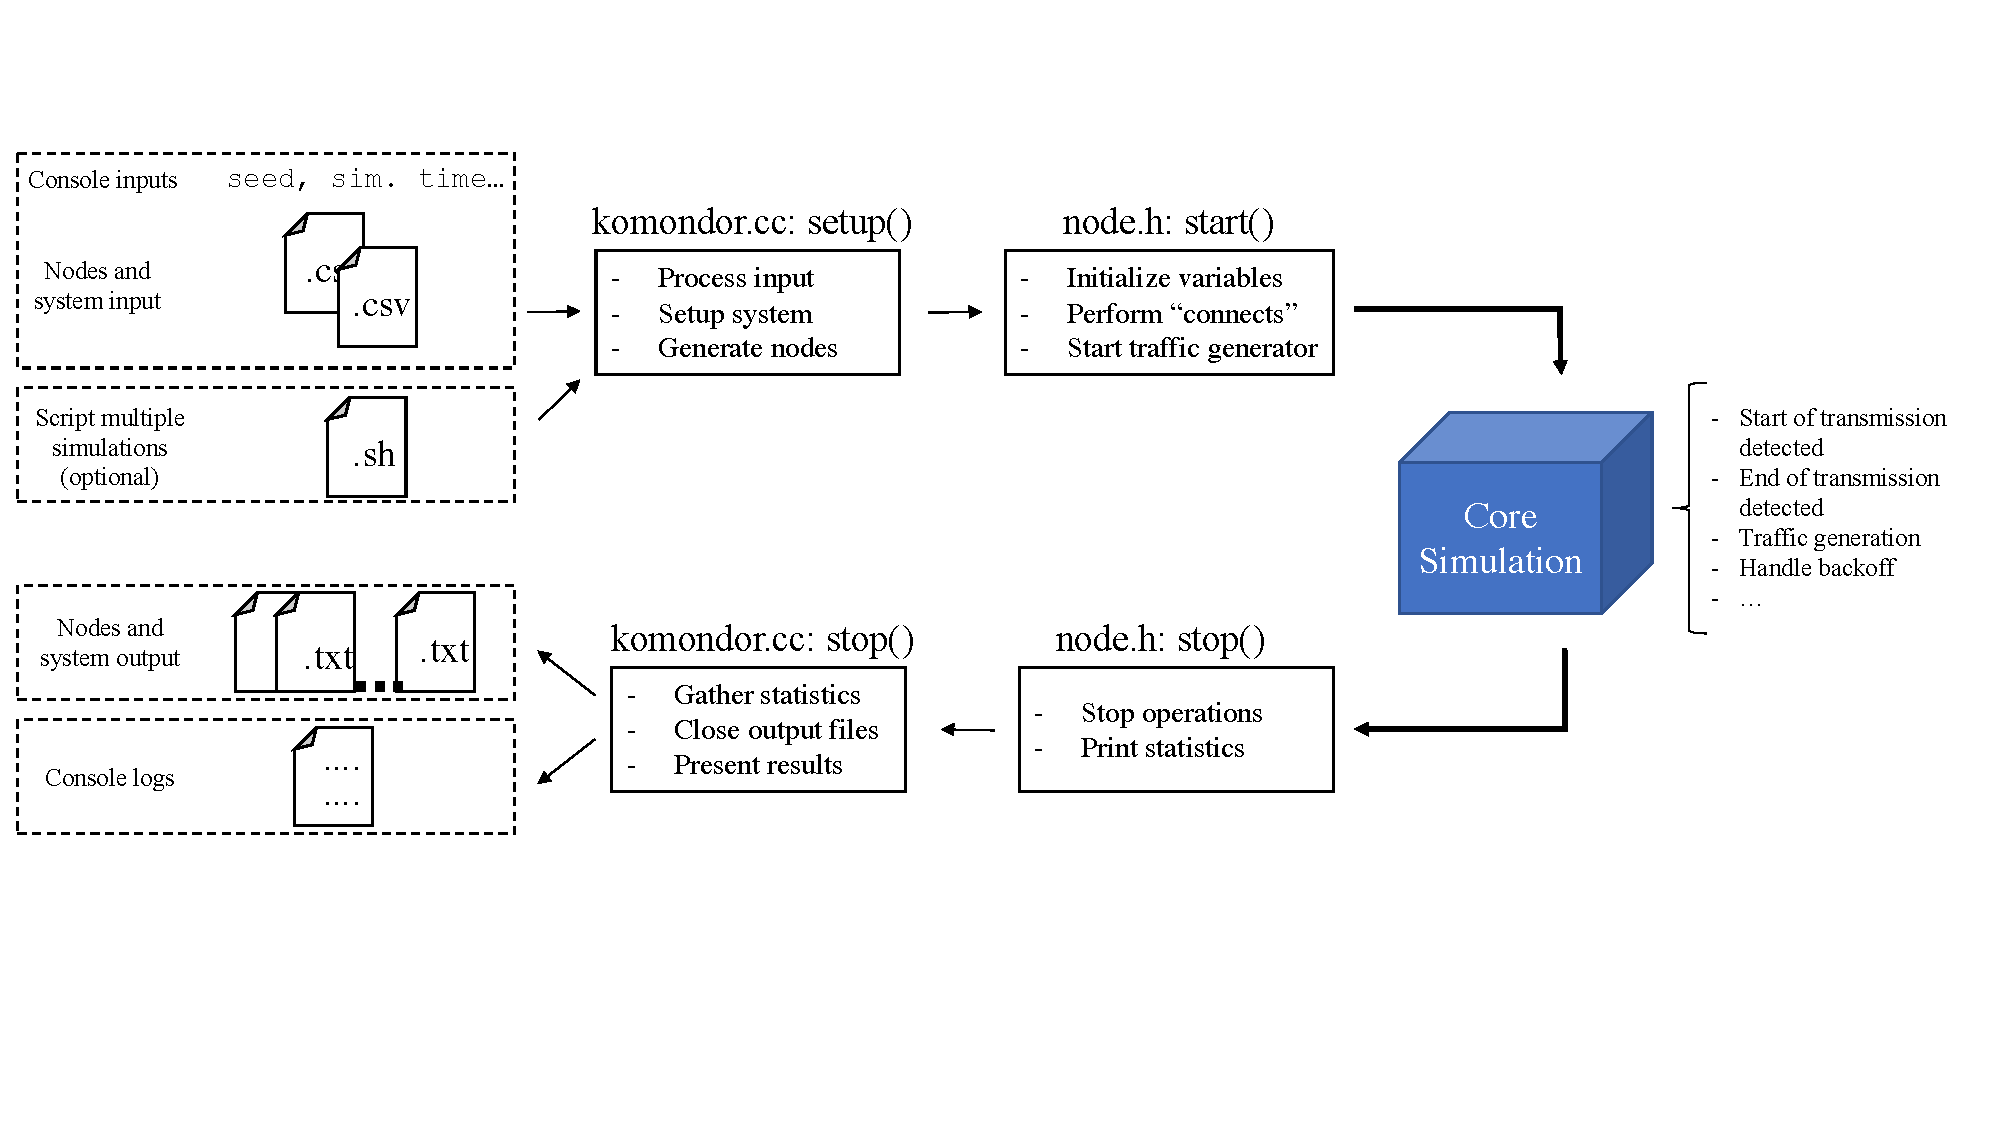
\epsfig{file=images/komondor_flowchart, width=15cm}
			\caption{Komondor flowchart}
			\label{fig:komondor_flowchart}
		\end{figure}		
		
		% Project organization
		\subsubsection{Files Organization}
		\label{section:files}		
		To properly understand the Komondor's operation, it is important to describe how the project is organized, which provides an overview of the different modules that constitute it. The code is organized as follows:
		\begin{itemize}
			\item COST libraries: contains the necessary COST libraries that allow the Komondor's primitive operation. 
			\item Code: contains the two core files, which are \emph{komondor.cc} and \emph{node.h}, which are in charge of orchestrating all the simulation. In addition, here we find the inputs and the file that compiles the libraries for executing the code (\emph{build\_local}).
			\item Methods: by following clean architecture guidelines, independent methods used by both \emph{komondor.cc} and \emph{node.h} files are contained in the methods folder. Several libraries are provided according to the nature of their functions. For instance, \emph{backoff\_methods.h} contains methods to handle the backoff operation.
			\item Structures: the Komondor simulator considers four main objects to carry out its operation. The first one is \emph{wlan.h}, which defines the main characteristics of a WLAN (WLAN id, list of associated STAs, etc.). Furthermore, the \emph{notification.h} object allows to exchange packets between devices. Finally, \emph{logger.h} and \emph{logical\_nack.h} are used for auxiliary purposes, which are displaying logs and saving packet losses causes, respectively.
			\item List of macros: all the static parameters are contained in the \emph{list\_of\_macros.h} file. 			
		\end{itemize}
		
		% Compilation & Execution
		\subsubsection{Compilation and Execution}
		\label{section:compilation_execution}
		To compile and execute a Komondor's simulation, the following instructions must	be followed:
		\begin{enumerate}
			\item Set the .csv input files (further defined in Section \ref{section:input_files})
			\item "cd" to \textit{KomondorSimulator} directory
		    \item Execute ".build\_local". This file contains the instructions for compiling the Komondor code. It has been updated to enable debugging with Valgrind\footnote{Valgrind is a programming tool for memory debugging, memory leak detection, and profiling. Valgrind main website: \url{http://valgrind.org/}}.
		    \item Execute \textit{./KomondorSimulator arg\_1 arg\_2 ... arg\_n}, where \textit{arg\_i} is the $i_{\text{th}}$ input argument:
		    	\begin{itemize}		            
		            \item \textit{arg\_1} (INPUT\_FILE\_SYSTEM\_CONFIGURATION): file containing system information (e.g., number of channels available, traffic model, etc.). The file must be a .csv with semicolons as separators.
		            \item \textit{arg\_2} (INPUT\_FILE\_NODES): file containing nodes information (e.g., position, channels allowed, etc.).The file must be a .csv with semicolons as separators.
		            \item \textit{arg\_3} (OUTPUT\_FILE\_LOGS): path to the output file to which write results at the end of the execution (if the file does not exist, the system will create it).
		            \item \textit{arg\_4} (FLAG\_SAVE\_SYSTEM\_LOGS): flag to indicate whether to save the system logs into a file (1) or not (0).\footnote{Major increases in the execution time may occur if nodes logging is activated. E.g., for a simulation of 4 nodes, simulating 1000 seconds takes 1.127 s and 15.672 s when not logging and when doing so, respectively.}
		            \item \textit{arg\_5} (FLAG\_SAVE\_NODE\_LOGS): flag to indicate whether to save the nodes logs into separate files (1) or not (0). If this flag is activated, one file per node will be created.
		            \item \textit{arg\_6} (FLAG\_PRINT\_SYSTEM\_LOGS): flag to indicate whether to print the system logs (1) or not (0).
		            \item \textit{arg\_7} (FLAG\_PRINT\_NODE\_LOGS): flag to indicate whether to print the nodes logs (1) or not (0).
		            \item \textit{arg\_8} (SIM\_TIME): simulation time in seconds.
		            \item \textit{arg\_8} (SEED): random seed for the experiments.
				\end{itemize}
		    \item Collect the results either in the output files or in the console.
		\end{enumerate}
	
		In case that the user does not have permissions to execute some of the files, grant them by introducing the following command in the target folder: \emph{\$ chmod -R 777 *}.
		
		Furthermore, in order to ease experimental procedures, we provide a mechanism for executing several simulations and properly collecting all the results. At folder ``scripts multiple executions" one can find few examples for executing a list of input files, thus generating several outputs.		
		
		% Input
		\subsubsection{Input files}
		\label{section:input_files}	
		The Komondor simulator relies in two types of input files for defining the simulation environment:
		\begin{itemize}
			\item \textbf{System input:} defines global input parameters such as packets length or propagation models. System input parameters are defined in Table \ref{table:system_parameters}.
			\item \textbf{Nodes input:} defines specific nodes' characteristics such as implementing features (e.g., CB policy). There are two ways of generating nodes, which is indicated in the file name. While including the keyword \emph{nodes} all the devices (APs and STAs) must be introduced and described. Otherwise, if including the keyword \emph{aps}, only the APs are defined, so that a STAs are randomly generated under certain introduced parameters (e.g., minimum/maximum number of STAs, maximum distance between APs and STA).\footnote{The usage of APs input files is discouraged to the lack of maintenance.} As a final remark, in order to ensure a proper execution, it is mandatory to introduce and input file with a list of nodes ordered by \textit{node\_id} and starting with \textit{node\_id} = 0. It is needed for the array responsible of storing the power perceived by each node (i.e., \textit{power\_received\_per\_node}). Table \ref{table:nodes_parameters} describes the Nodes input parameters for both \emph{nodes} and \emph{aps} files.
		\end{itemize}		

		%  System input parameters	
		\begin{table}[h!]
			\centering
			\begin{tabular}{|c|c|l|}
				\hline
				\textbf{Parameter} & \textbf{Type} & \multicolumn{1}{c|}{\textbf{Description}} \\ \hline
				num\_channels & int & \begin{tabular}[c]{@{}l@{}}Maximum number of frequency channels \\ in the system\end{tabular} \\ \hline
				basic\_channel\_bandwidth & int & Bandwidth for each channel {[}MHz{]} \\ \hline
				pdf\_backoff & int & PDF to compute the backoff () \\ \hline
				pdf\_tx\_time & int & PDF to compute the tx time () \\ \hline
				packet\_length & int & Length of data packets {[}bits{]} \\ \hline
				ack\_length & int & Length of ACK packets {[}bits{]} \\ \hline
				num\_packets\_aggregated & int & Number of packets aggregated per transmission \\ \hline
				path\_loss\_model & int & \begin{tabular}[c]{@{}l@{}}Path-loss model (0: FSPL, 1: Hata, \\ 2: Indoor 1, 3: Indoor 2, 4: TGax scenario 1)\end{tabular} \\ \hline
				capture\_effect & int & Capture Effect Threshold {[}dB{]} \\ \hline
				noise\_level & int & Floor noise level {[}dBm{]} \\ \hline
				adjacent\_channel\_model & int & \begin{tabular}[c]{@{}l@{}}Co-channel interference model \\ (0: without adjacent interference,\\ 1: contiguous adjacent interference, \\ 2: complete adjacent interference)\end{tabular} \\ \hline
				collisions\_model & int & Collisions model (reserved) \\ \hline
				SIFS & int & SIFS period {[}$\mu$s{]} \\ \hline
				constant\_PER & int & Defines a constant Packet Error Rate \\ \hline
				traffic\_model & int & \begin{tabular}[c]{@{}l@{}}Traffic model (0: full buffer, 1: Poisson distr., \\ 2: deterministic distr.)\end{tabular} \\ \hline
				backoff\_type & int & Type of backoff (discrete: 0, continuous: 1) \\ \hline
				rts\_length & int & Length of RTS packets {[}bits{]} \\ \hline
				cts\_length & int & Length of CTS packets {[}bits{]} \\ \hline
				cw\_adaptation & bool & For activating CW adaptation \\ \hline
				pifs\_activated & bool & For activating PIFS \\ \hline
			\end{tabular}
			\caption{System input parameters description}
			\label{table:system_parameters}
		\end{table}
		
		% Nodes input parameters		
		\begin{table}[h!]
			\centering
			\begin{tabular}{|c|c|c|l|}
				\hline
				\textbf{Parameter} & \textbf{Type} & \textbf{Nodes or APs} & \multicolumn{1}{c|}{\textbf{Description}} \\ \hline
				node\_code & String & nodes & Code assigned to the node \\ \hline
				node\_type & int & nodes & Type of node (0: AP, 1: STA) \\ \hline
				wlan\_code & String & both & Code assigned to the WLAN \\ \hline
				destination\_id & int & nodes & \begin{tabular}[c]{@{}l@{}}To specify the ID of the destination \\ (packets would be only sent to that devices).\\ Setting it to -1 specifies current operation.\end{tabular} \\ \hline
				min\_sta\_number & int & aps & Minimum number of associated STAs \\ \hline
				max\_sta\_number & int & aps & Maximum number of associated STAs \\ \hline
				max\_distance\_sta & int & aps & Maximum distance of associated STAs \\ \hline
				x & int & both & X location {[}m{]} \\ \hline
				y & int & both & Y location {[}m{]} \\ \hline
				z & int & both & Z location {[}m{]} \\ \hline
				primary\_channel & int & both & Primary channel \\ \hline
				min\_channel\_allowed & int & both & Left channel in range \\ \hline
				max\_channel\_allowed & int & both & Right channel in range \\ \hline
				cw & int & both & Fixed CW \\ \hline
				cw\_stage & int & both & Initial CW stage (for CW adaptation) \\ \hline
				tpc\_min & int & both & Minimum transmit power allowed {[}dBm{]} \\ \hline
				tpc\_default & int & both & Default transmit power allowed {[}dBm{]} \\ \hline
				tpc\_max & int & both & Maximum transmit power allowed {[}dBm{]} \\ \hline
				cca\_min & double & both & Minimum CCA allowed {[}dBm{]} \\ \hline
				cca\_default & double & both & Default CCA allowed {[}dBm{]} \\ \hline
				cca\_max & double & both & Maximum CCA allowed {[}dBm{]} \\ \hline
				tx\_antenna\_gain & int & both & Gain of the tx antenna {[}dB{]} \\ \hline
				rx\_antenna\_gain & int & both & Gain of the rx antenna {[}dB{]} \\ \hline
				channel\_bonding\_model & int & both & \begin{tabular}[c]{@{}l@{}}Channel bonding model (0: only primary, \\ 1: SCB, 2: SCB log2, 3: always max, \\ 4: always max log2, 5: always max log2 MCS,\\ 6: uniform probability log2)\end{tabular} \\ \hline
				modulation\_default & int & both & \begin{tabular}[c]{@{}l@{}}Modulation set by default \\ (0 to use dynamic MCS)\end{tabular} \\ \hline
				central\_freq & int & both & Frequency band used (2,4 or 5 GHz) \\ \hline
				lambda & float & both & Packets transmission rate {[}packets/s{]} \\ \hline
				ieee\_protocol & int & both & IEEE protocol used \\ \hline
			\end{tabular}
			\caption{Nodes input parameters description}
			\label{table:nodes_parameters}
		\end{table}
		
		% Output
		\subsubsection{Output files}
		\label{section:output_files}	
		A lot of effort has been put on the output generation, since it is a sensitive module that allows understanding and validating the results provided by the simulator. Henceforth, we provide different kinds of outputs, which refer to console and file output logs. Note, as well, that generating output files considerably increases the computation time. 
		
		Regarding console output logs, them can be activated through \emph{arg\_6} and \emph{arg\_7} during the execution, which refer to system and nodes logs, respectively (see Section \ref{section:compilation_execution}). Additionally, those logs can be copied into files, which are saved into the \emph{output} folder, only if \emph{arg\_4} and \emph{arg\_5} are set to 1. While the path of the system's output file must be specified (\emph{arg\_3}), nodes' files are automatically created. 
		
		Finally, a set of statistics are show per node and for the entire simulation. Such statistics include throughput experienced, collisions, nodes sent, RTS/CTS sent, etc. An example of nodes and system statistics is shown in Figures \ref{fig:nodes_statistics_example} and \ref{fig:general_statistics_example}
		\begin{figure}[h!]
			\centering
			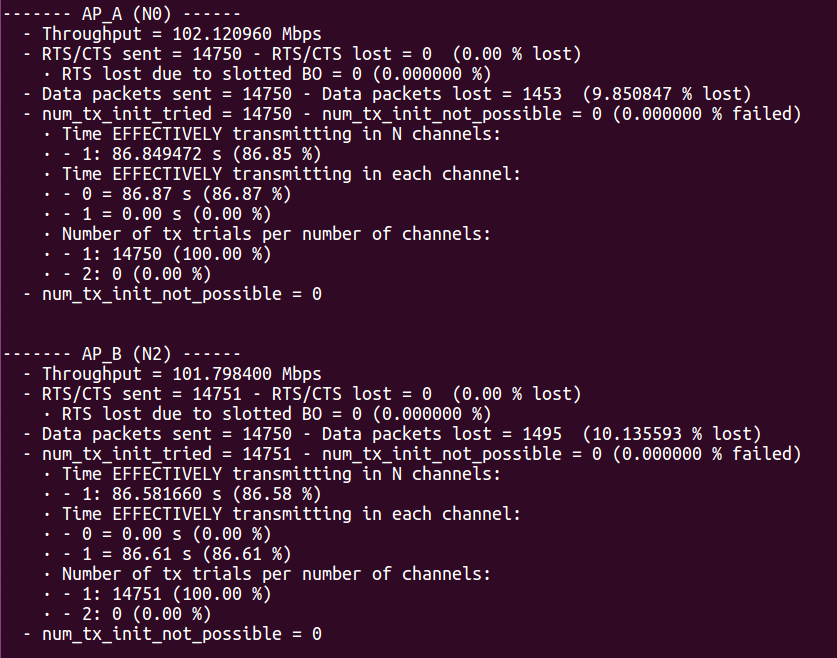
\epsfig{file=images/nodes_statistics_example, width=12cm}
			\caption{Example of nodes statistics in Komondor}
			\label{fig:nodes_statistics_example}
		\end{figure}
		
		\begin{figure}[h!]
			\centering
			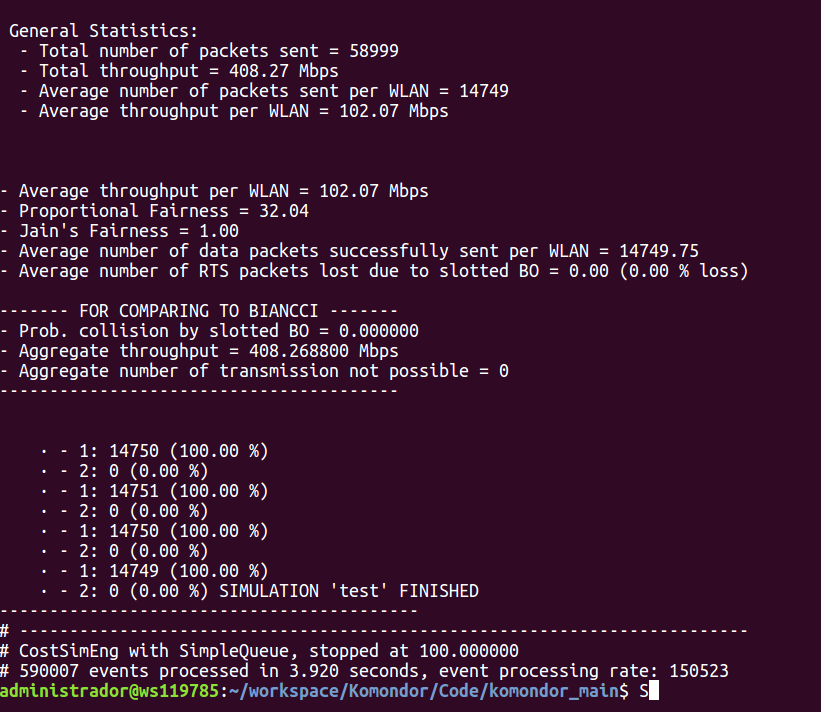
\epsfig{file=images/general_statistics_example, width=12cm}
			\caption{Example of system statistics in Komondor}
			\label{fig:general_statistics_example}
		\end{figure}
	
		% Logs system
		\subsubsection{Events Categorization}
		\label{section:events_categorization}	
		In order to provide a better understanding when reviewing the results of a given execution, logs are categorized according to the event that generates it. With that, further filtering processes can be carried out by developers. Table \ref{table:event_coding} describes the codes used for each type of event.		
		% Events coding table
		\begin{table}[]
		\centering
		\scriptsize
		\begin{tabular}{|c|c|c|c|}
		\hline
		\textbf{Method}                            & \textbf{Type}       & \textbf{Sub-type} & \textbf{Event description}                              \\ \hline
		Setup()                                    & A                   & -                 & -                                                       \\ \hline
		\multirow{3}{*}{Start()}                   & \multirow{3}{*}{B}  & B00               & Start()                                                 \\ \cline{3-4} 
		                                           &                     & B01               & Start() end                                             \\ \cline{3-4} 
		                                           &                     & B02               & Node's info (one line)                                  \\ \hline
		\multirow{6}{*}{Stop()}                    & \multirow{6}{*}{C}  & C00               & Stop()                                                  \\ \cline{3-4} 
		                                           &                     & C01               & Stop() end                                              \\ \cline{3-4} 
		                                           &                     & C02               & Time transmitting in number of channels                 \\ \cline{3-4} 
		                                           &                     & C03               & Time transmitting in each channel                       \\ \cline{3-4} 
		                                           &                     & C04               & Packets sent                                            \\ \cline{3-4} 
		                                           &                     & C05               & Throughput                                              \\ \hline
		\multirow{14}{*}{inportSomeNodeStartTX()}  & \multirow{14}{*}{D} & D00               & inportSomeNodeStartTX()                                 \\ \cline{3-4} 
		                                           &                     & D01               & inportSomeNodeStartTX() end                             \\ \cline{3-4} 
		                                           &                     & D02               & Node N has started a TX in channels: c\_left - c\_right \\ \cline{3-4} 
		                                           &                     & D03               & Pre update channel state                                \\ \cline{3-4} 
		                                           &                     & D04               & Distance to transmitting node                           \\ \cline{3-4} 
		                                           &                     & D05               & Power received from transmitting node                   \\ \cline{3-4} 
		                                           &                     & D06               & Post update channel state                               \\ \cline{3-4} 
		                                           &                     & D07               & I am (or not) the TX destination                        \\ \cline{3-4} 
		                                           &                     & D08               & Current SINR                                            \\ \cline{3-4} 
		                                           &                     & D09               & Capacitiy                                               \\ \cline{3-4} 
		                                           &                     & D10               & Primary channel affected (or not)                       \\ \cline{3-4} 
		                                           &                     & D11               & Power sensed in primary channel                         \\ \cline{3-4} 
		                                           &                     & D12               & CCA exceeded (or not)                                   \\ \cline{3-4} 
		                                           &                     & D13               & Backoof active (or not)                                 \\ \hline
		\multirow{10}{*}{inportSomeNodeFinishTX()} & \multirow{10}{*}{E} & E00               & inportSomeNodeFinishTX()                                \\ \cline{3-4} 
		                                           &                     & E01               & inportSomeNodeFinishTX() end                            \\ \cline{3-4} 
		                                           &                     & E02               & N\%d has finished a TX in channel range: \%d - \%d      \\ \cline{3-4} 
		                                           &                     & E03               & Initial power of transmitter                            \\ \cline{3-4} 
		                                           &                     & E04               & Pre update channel state                                \\ \cline{3-4} 
		                                           &                     & E05               & Post update channel state                               \\ \cline{3-4} 
		                                           &                     & E06               & Primary channel affected (or not)                       \\ \cline{3-4} 
		                                           &                     & E07               & Power sensed in primary channel                         \\ \cline{3-4} 
		                                           &                     & E08               & CCA exceeded (or not)                                   \\ \cline{3-4} 
		                                           &                     & E09               & I am transmitting (or not)                              \\ \hline
		\multirow{6}{*}{endBackoff()}              & \multirow{6}{*}{F}  & F00               & endBackoff()                                            \\ \cline{3-4} 
		                                           &                     & F01               & endBackoff() end                                        \\ \cline{3-4} 
		                                           &                     & F02               & Channels for transmitting                               \\ \cline{3-4} 
		                                           &                     & F03               & Transmission is possible (or not)                       \\ \cline{3-4} 
		                                           &                     & F04               & Selected transmission range                             \\ \cline{3-4} 
		                                           &                     & F05               & New backoff generated                                   \\ \hline
		\multirow{3}{*}{myTXFinished()}            & \multirow{3}{*}{G}  & G00               & myTXFinished()                                          \\ \cline{3-4} 
		                                           &                     & G01               & myTXFinished() end                                      \\ \cline{3-4} 
		                                           &                     & G02               & New backoff generated                                   \\ \hline
		\end{tabular}
		\caption{Node's event logs encoding}
		\label{table:event_coding}
		\end{table}

	%%% Code Development
	\subsection{Code development}
	\label{section:code_development}		
	This Section is mostly focused in providing the most important clarifications regarding the code to developers that may be interested in using and/or modifying the presented simulator.
	
		% Considerations
		\subsubsection{Main considerations}
		\label{section:development_considerations}
		% TODO: Extend this part.
		Some technical information regarding code development is worth to be mentioned to properly understand how to use and modify the Komondor simulator. So far, the main considerations to be taken into account are:		
		\begin{itemize}
		\item \textbf{Power and CCA}: power variables are stored in pW (pico watts) in order to be able to operate power magnitudes without loosing resolution\footnote{For instance., the sum of two signals of power values -85 dBm (3.162 pW) and -90 dBm (1 pW), respectively, is -83.803 dBm (4.162 pW).}. However, values are presented to the user in dBm.		
		W (-30)  - mW (0)  - uW (+30) - nW (+60) - pW (+90)\\
		$P_{\text{pw}} = 10^{\frac{P_{\text{dBm}} + 90}{10}}$
		\end{itemize}
	
		% Miscellany
		\subsubsection{Miscellany}
		\label{section:development_miscellany}
		% TODO: Extend this part.
			\begin{itemize}
			\item Transmitting capability: we have added a flag to each node that determines if it is able to transmit (1) or not (0), so that we can decide if the node is only listening or both transmitting and listening.
			\item Progress bar: the Komondor simulation progress bar is displayed through a \textit{printf()} command called by any node with \textit{node\_id} set to 0. If no node has \textit{node\_id} set to 0, the progress bar is not displayed.
			\end{itemize}
	
		% Miscellany
		\subsubsection{Releases}
		\label{section:development_releases}
		% TODO: Decide to include this section or not. If yes, extend it.
		So far, Komondor has experienced two main releases. The first one, Komondor v0.1, included a basic operation in which only data packets were exchanged. Such version included the following features:
		\begin{itemize}
			\item Channel Bonding
			\item Adjacent power
			\item Collisions
			\item Scripting
			\item Path loss models
		\end{itemize}
	
		Furthermore, the release presented in this document, Komondor v1.0, extends the basic operation of v0.1 and includes all the features previously described.

%%%%%%%%%%%%%%%
% 6. CONCLUSIONS
%%%%%%%%%%%%%%%
\section{Conclusions}
\label{section:conclusions}
In this document we provided an overview of the first version of the Komondor simulator, which aims to reproduce the basic operation of IEEE 802.11ax WLANs in addition to allow the utilization of intelligent systems. We provided the system model considered when building the simulator, as well as the main MAC features implemented. Additionally, due to the open source nature of this project, we provided basic information of interest for developers that are expected to use or even modify this networks simulator.

Regarding validations, we provided a set of meaningful test scenarios to prove the proper behavior of the simulator. As shown,  tests were satisfactory as the throughput computed with Komondor and the CTMN model are pretty similar.

This project is expected to move forward for including of novel mechanisms such as OFDMA, MU-MIMO, TPC or  CST adjustment. In addition, intelligent agents are expected to be included for making operations such as Dynamic CB (DCB).

%%% BIBLIOGRAPHY
\bibliographystyle{unsrt}
\bibliography{bib}

\end{document}